\documentclass[main.tex]{subfiles}

\begin{document}

\chapter{Sole, Terra, stelle, pianeti: dimensioni caratteristiche}
\PartialToc

\section{Sole}

\subsection{Massa e densit\'a}
\begin{itemize*}
\item $\msun\approx1.989*10^{30}\,Kg$
\item $\rhosun\approx1.408 \, gr/cm^3$
\end{itemize*}

\begin{itemize*}
\item $\rsun=6.96*10^8\,m$
\end{itemize*}
\begin{itemize*}
\item $\msun\approx1.989*10^{30}\,Kg$
\item $\rhosun\approx1.408 \, gr/cm^3$
\end{itemize*}

\subsection{G-nal potential energy}

\begin{equation*}
\Omega=\frac{G\msun^2}{\rsun}\approx\num{3.8e48}\si{\erg}
\end{equation*}

\subsection{superficie}

\begin{itemize*}
\item $\gsun=\frac{G\msun}{\rsun^2}=274\,m/s^2$
\end{itemize*}

\subsection{Solar constant}

Solar radiation constant at \SI{1}{\astronomicalunit}
\begin{align*}
&F_0=\SI{1.366e7}{\erg\per\square\cm\per\second}\\
&=\SI{1.366e3}{\joule\per\square\meter\per\second}
\end{align*}


\section{Terra}


\subsection{Massa e densit\'a}

\begin{equation*}
\mT=5.972\sci{27}\,g=5.972\sci{24}\,Kg
\end{equation*}

\subsection{Mean Earth radius}

\begin{equation*}
\rT=6.371\sci{8}\,cm=6.371\sci{6}m
\end{equation*}

\subsection{Oblateness coefficient}

\begin{equation*}
J_2=\frac{C-A}{\mT\rT^2}
\end{equation*}


\subsection{Obliquity at standard epoch}

\begin{align*}
\epsilon=\ang{23;26;21}&\intertext{At standard epoch $J2000.0$}
\end{align*}

\subsection{Lunisolar precession constant}
Rate at which the the vernal equinox point or $gamma$ point intersection between the celestial equator and ecliptic moves along the latter
\begin{equation*}
\Omega_{pr}=\ang{;;50.291}/yr=7.726\sci{-12}\,rad/s
\end{equation*}

\subsection{Sideral angular velocity and secular decreases}

Rotation of Earth on its axis.

\begin{align*}
\roT=(7.2921\sci{-5}-1.4\sci{-14}T)\si{\radian \per \second}&\intertext{T in years}
\end{align*}


 
\section{Masse e densit\'a caratteristiche}

\subsection{White dwarf}

\subsection{Galaxy}


\section{Angoli}

\begin{itemize*}
\item arcosecondo $1''=4.848\sci{-6}\,rad$
\item 1 degree ($\degree$) = \ang{;60;} = \ang{;;3600}
\item \SI{1}{\radian} = \ang{57.296;;} = \ang{;;206265}
\item \SI{1}{\steradian} = \SI{1}{\square\radian} = \SI{3282.8}{\square\deg} = \SI{4.25e10}{\square\arcsec}, where $4\pi$ steradians is the sphere.

\end{itemize*}


\section{Stelle}


\chapter{Energie, frequenze, lunghezze:unit\'a di misura.}
\PartialToc

\section{Unit\'a di misura}

\subsection{Energia}

\begin{align*}
\si{\erg=\dyn\cm}
\end{align*}

\begin{equation*}
1\,erg = 624.15\,GeV = 6.2415*10^{11}\, eV
\end{equation*}

\begin{align*}
&1\,eV=1.602\sci{-12}\,erg\\
&=1.602\sci{-19}\,J=11600\,K\\
\end{align*}

\begin{align*}
1  ^{\degree}K&= 8.621738*10^{-5}  eV \\
&= 0.0862 meV \\
&= 0.695 cm^{-1}
\end{align*}

\begin{align*}
&1 a.u=27.211396 eV=219474.63 cm^{-1}\\
&1 Ry=13.6057 eV \\
&1 eV =8065.54 cm^{-1} \\
&1 eV= 11,600  ^{\degree}K\\
&1 meV = 8.065 cm^{-1}
\end{align*}

\subsection{Relazioni $u,c,MeV$}
 
\begin{align*}
&c^2=931.502\frac{MeV}{u}
&1 u=931.49 \Mcs
\end{align*}
 

\subsection{Astronomical unit}

Mean heliocentric distance of Earth.
\begin{equation*}
1\,AU=1.496\sci{13}\,cm=1.496\sci{11}\,m
\end{equation*}

\subsection{ly/cm/m}

\begin{equation*}
1\,ly=9.46\sci{17}cm=9.46\sci{15}m
\end{equation*}

\subsection{parsec/UA/cm/ly}

\begin{align*}
&1\,pc=\frac{\SI{1}{\astronomicalunit}}{(\frac{1}{60*60}*\frac{\pi}{180})}=\frac{648000}{\pi}\,UA\\
&\approx\SI{2e5}{\astronomicalunit}=3.086\sci{18}\,cm\\
&=3.086\sci{16}\,m=3.26\,ly
\end{align*}

\section{Costante di Boltzmann $k$}


\begin{align*}
&k=1.381\sci{-16}\,erg/K=1.381\sci{-23}\,J/K\\
&k=\SI{1.3805e-16}{\erg\per\kelvin}\\
&k=\SI{8.617e-5}{\ev\per\kelvin}\\
&\frac{k}{h}=\SI{2,0836618e10}{\hertz\per\kelvin}
\end{align*}

\section{Lunghezza Compton elettrone}

The Compton wavelength is a quantum mechanical property of a particle. It was introduced by Arthur Compton in his explanation of the scattering of photons by electrons (a process known as Compton scattering). The Compton wavelength of a particle is equivalent to the wavelength of a photon whose energy is the same as the rest-mass energy of the particle.

\begin{align*}
&\lambda_c=\frac{h}{m_ec}=\SI{2.426e-10}{\cm}
\end{align*}


\section{Radiazione.}

\begin{tabular}{ccc}
Region &  $\lambda$ & Energy\\
RF&$>\SI{1}{\meter}$ & $<\SI{e-5}{\ev}$\\
mw,mm & $1-0.0003\si{\meter}$&\SIrange{e-2}{e-5}{\ev}\\
visible&$700-400nm$&$1.77-3.1\si{\ev}$\\
UV&$400-10nm$&$3.1-120 \si{\ev}$\\
X-ray&$<10nm$&$>120 \si{\ev}$\\
\end{tabular}

\subsection{Costante di Plank}

\begin{equation*}
h=6.626\sci{-27}\,erg\,s=6.626\sci{-34}\,J\,s
\end{equation*}

\subsection{Costante di Stefan-Boltzmann}

\begin{align*}
&\sigma=\frac{2\pi^5k^4}{15c^2h^3}=5.67\sci{-5}\,erg/cm^2/s/K^4\\
&=5.67\sci{-8}\,W/m^2/K^4
\end{align*}

\subsection{Radiation density constant}

\mblock{u=aT^4} con \mblock{a=\SI{7.57e-15}{\erg\per\cubic\cm\per\kelvin\tothe{4}}}


\section{Costante di gravitazione universale.}

\begin{align*}
&G=6.674\sci{-8}\,dyne\,cm^2\,g^{-2}\\
&=6.674\sci{-11}\,N\,m^2\,Kg^{-2}
\end{align*}


\section{Gravitational field}

\subsection{Local gravity at spherical radius}
\begin{equation*}
g(r)=\frac{Gm(r)}{r^2}=2.74\sci{4}(\frac{m(r)}{\msun})(\frac{r}{\rsun})^{-2}\si{\cm\per\square\second}
\end{equation*}


\section{Costanti di conversione}

\subsection{Angstrom-nanometer}
\begin{equation*}
\SI{1}{\angstrom}=\SI{e-8}{\cm}=\SI{0.1}{\nano\meter}
\end{equation*}

\section{Plasma}

\subsection{Lunghezza di Debye}

\begin{equation*}
\lambda_D=(\frac{kT}{4\pi e^2n_e})\expy{-\frac{1}{2}}=743(\frac{T}{n_e\,eV\,cm^3})\expy{\frac{1}{2}}\,cm
\end{equation*}

\subsection{Plasma frequencies}
Caratterizza l'effetto delplasma sulla propagazione di onde elettromagnetiche. Il plasma \'e trasparente per $\omega\gg\omega_P$.

\begin{equation*}
\omega_P=\sqrt{\frac{4\pi n_ee^2}{m_e}}=56400\sqrt{n_e\,cm^3}\,rad/s
\end{equation*}

\subsection{Cyclotron frequency}

Il moto di un'elettrone in un campo magnetico \'e caratterizzato dalla frequenza di ciclotrone
\begin{equation*}
\Omega_e=\frac{eB}{m_ec}=1.76\sci{7}\frac{B}{\sci{5}\,nT}\,rad/s
\end{equation*}
per gli ioni con $m_i=Am_p$, ho la rispettiva frequenza
\begin{equation*}
\Omega_i=\frac{ZeB}{m_ic}=9580\frac{Z}{A}\frac{B}{\sci{5}\,nT}\,rad/s
\end{equation*}

\subsection{Grandezze nucleari}

\begin{align*}
&fm=\SI{e-15}{\meter}=\SI{e-13}{\cm}\\
&\si{\angstrom}=\SI{e-8}{\cm}
\end{align*}

\chapter{Thermodynamic constant}
\PartialToc

\section{"Chemical" masses}

\subsection{Mole of matter, atomic mass unit}
\begin{align*}
&1\si{\mole}=\# \text{atoms in }0.012\si{\kilo\gram}\text{ of $^{12}C$}\\
&N_A*12 \si{\atomicmassunit}=0.012\si{\kilo\gram\per\mole}\\
&1\si{\atomicmassunit}=\frac{1\si{\gram\per\mole}}{N_A}\approx m_p
\end{align*}

\subsection{Avogadro constant}
\begin{align*}
N_A=\num{6.022e23}\si{\per\mole}
\end{align*}

\subsection{Atomic mass unit}

\si{\atomicmassunit} is defined so that an atom of $^{12}C$ has mass $12 \si{\atomicmassunit}$, $N_A$ is number of $^{12}C$ in $12 \si{\gram}$ of $^{12}C$ and a \si{\mole} is the amount of substance in a system that contains as many atoms as there are atoms in $12\si{\gram}$ of $^{12}C$.



\section{Gas}

\subsection{Universal Gas constant R}

It is equivalent to the Boltzmann constant, but expressed in units of energy (i.e. the pressure-volume product) per temperature increment per mole (rather than energy per temperature increment per particle).

\begin{align*}
&k=\frac{\gasconstant{}}{N_A}=8.617\,eV/K\\
&R=k/m_u=8.31*10^7 \si{\erg\per\kelvin\per\gram}\\
&R=8.31\,J/mol/K
\end{align*}

\subsection{specific gas constant.}

The specific gas constant of a gas or a mixture of gases ($R_{Specific}$) is given by the molar gas constant divided by the molar mass (M) of the gas/mixture.

Just as the ideal gas constant can be related to the Boltzmann constant, so can the specific gas constant by dividing the Boltzmann constant by the molecular mass of the gas.

Another important relationship comes from thermodynamics. Mayer's relation relates the specific gas constant to the specific heats for a calorically perfect gas and a thermally perfect gas.

\begin{align*}
&R_{specific} = \frac{R}{M}\\
&R_{specific} = \frac{{k_{B}}}{m}\\
&R_{specific} = c_p - c_v
\end{align*}

where $c_p$ is the specific heat for a constant pressure and $c_v$ is the specific heat for a constant volume.

In any case, the context and/or units of the gas constant should make it clear as to whether the universal or specific gas constant is being referred to.
 
\chapter{Costanti fisica atomica e nucleare}
\PartialToc

\section{Particelle fondamentali}

\begin{itemize*}
\item $m_P=938.3\Mcs$
\item $m_P=\SI{1.672 621 898+-0.000 000 021e-27}{\kilo\gram}$
\item $m_N=939.7\Mcs$
\item $m_e=0.51\Mcs$
\item $r_e=\SI{2.817 940 3227+-0.000 000 0019e-15}{\meter}$.

\begin{definition}{Classical electron radius}
\begin{equation*}
r_e=(\frac{1}{4\pi\epsilon_0})\frac{e^2}{m_ec^2}
\end{equation*}
\end{definition}
\end{itemize*}



\section{Costante struttura fine}
 
 $\alpha_{SF}=\frac{e^2}{(4\pi\epsilon_0)\hbar c}$.

The ratio of three characteristic lengths:

the classical electron radius $r_e=(\frac{1}{4\pi\epsilon_0})\frac{e^2}{m_ec^2}$, the Bohr radius $a_0=(4\pi\epsilon_0)\frac{\hbar^2}{m_ee^2}$  and the Compton wavelength of the electron $\lambdabar_e=\frac{\hbar}{m_ec}$:

$r_e=\frac{\alpha\lambda_e}{2\pi}=\alpha^2a_0$.

$e^2=1.44\,MeV\,fm$


\section{Nuclei}

\subsection{Magnetone nucleare}
 
\begin{equation*}
\frac{e\hbar}{2m_pc}=\mu_N=\frac{\mu_B}{1836}
\end{equation*}
 
\subsection{Deutone}
 
\begin{align*}
&B=2.22 MeV\\
&\mu_d=0.8574376\mu_N\\
&S=1\\
&Q=2.8*10^{-27}cm^2=0.28fm^2(Q_{zz}\\
&=\frac{2}{5}eZ(b^2-a^2))
\end{align*}
 
\section{Atomi}

\subsection{Atomo d'idrogeno}

\begin{align*}
&E_n=\frac{m_ec^2\alpha^2}{2n^2}=\frac{13.6eV}{n^2}\\
&a_0=\frac{\hbar}{m_ec\alpha}
 \end{align*}

\section{Energie ionizzazione}
 
\begin{todo}{Energie di ionizzazione}
Plot tabella in preamble
\end{todo}

\part{Mathematical Backgroung}

\chapter{Differential operators}
\PartialToc

\section{Divergenza, gradiente, rotore, laplaciano}

\begin{usefull}{Gradiente in coordinate sferiche}
\begin{align*}
\nabla f=\frac{\partial f}{\partial r}\hat{r}+\frac{1}{r}\frac{\partial f}{\partial \theta}\hat{\theta}+\frac{1}{r\sin{\theta}}\frac{\partial f}{\partial \phi}\hat{\phi}    
\end{align*}
\end{usefull}

\begin{usefull}{Divergenza in coordinate sferiche}
\begin{align*}
&\nabla\cdot\vec{A}=\frac{1}{r^2}\frac{\partial}{\partial r}(r^2A_r)+\frac{1}{r\sin{\theta}}\frac{\partial }{\partial \theta}(\sin{\theta}A_{\theta})\\
&+\frac{1}{r\sin{\theta}}\frac{\partial A_{\phi}}{\partial \phi}
\end{align*}
\end{usefull}

\begin{usefull}{Rotore in coordinate sferiche}
\begin{align*}
&\nabla\wedge\vec{A}=\frac{1}{r\sin{\theta}}(\frac{\partial}{\partial \theta}(A_{\phi}\sin{\theta})-\frac{\partial A_{\theta}}{\partial \phi})\hat{r}\\
&+\frac{1}{r}(\frac{1}{\sin{\theta}}\frac{\partial A_r}{\partial \phi}-\frac{\partial}{\partial r}(rA_{\phi}))\hat{\theta}\\
&+\frac{1}{r}(\frac{\partial}{\partial r}(rA_{\theta})-\frac{\partial A_r}{\partial \theta})\hat{\phi}
\end{align*}
\end{usefull}

\begin{usefull}{Laplaciano in coordinate sferiche}
\begin{align*}
&\nabla^2f=\frac{1}{r^2}\frac{\partial}{\partial r}(r^2\frac{\partial f}{\partial r})+\frac{1}{r^2\sin{\theta}}\frac{\partial}{\partial \theta}(\sin{\theta}\frac{\partial f}{\partial \theta})\\
&+\frac{1}{r^2\sin^2{\theta}}\frac{\partial^2f}{\partial \phi^2}=(\frac{\partial^2}{\partial r^2}+\frac{2}{r}\frac{\partial}{\partial r})f\\
&+\frac{1}{r^2\sin{\theta}}\frac{\partial}{\partial\theta}(\sin{\theta}\frac{\partial}{\partial \theta})f+\frac{1}{r^2\sin^2{\theta}}\frac{\partial^2}{\partial \phi^2}f
\end{align*}

\end{usefull}

\chapter{Shape: 2D, 3D. Surfaces, volumes, etc.}
\PartialToc

\section{Coniche}

equazione canonica:
\begin{equation*}
c_1x^2+c_2y^2+c_3=0
\end{equation*}

Le coniche devono il loro nome al fatto che sono ottenibili sezionando un cono doppio mediante un piano: se $\alpha$ \'e l'angolo tra l'asse e una retta generatrice del cono e $\beta$ l'angolo che la normale al piano secante forma con l'asse del cono, avremo
\begin{itemize}
\item Una sezione ellittica se \mblock{0<\beta<\alpha}.
\item Una sezione parabolica se $\beta=\alpha$.
\item Una sezione iperbolica se \mblock{\alpha<\beta<\frac{\pi}{2}}
\end{itemize}

\subsection{Ellipse}

\begin{align*}
&(\frac{x}{a})^2+(\frac{y}{b})^2=1\\
&x=a\cos{\theta},\ y=b\sin{\theta}\\
&(PF_1+PF_2=2a)\\
&0<\frac{a}{b}<1\\
&\epsilon=1-\frac{b}{a}&\intu{ellitticit\'a}\\
&e=\sqrt{1-\frac{b^2}{a^2}}&\intu{eccentricit\'a}\\
&r=\frac{p}{1+e\cos{\theta}},\ p=a(1-e^2)>0\\
&A=\pi ab
\end{align*}

\begin{figure}[!ht]
\centering
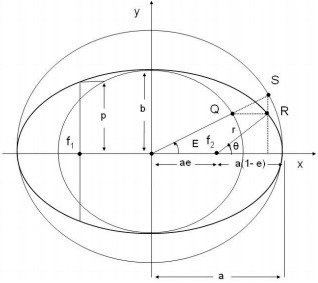
\includegraphics[width=(0.9\textwidth),height=(\textheight),keepaspectratio]{ellipse}
\caption{Ellisse.}
\end{figure}

\clearpage


\subsection{Parabola}

\begin{figure}[!ht]
\centering
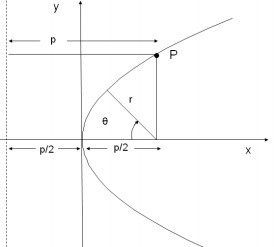
\includegraphics[width=(0.9\textwidth),height=(\textheight),keepaspectratio]{parable}
\caption{Parabola.}
\end{figure}

\begin{align*}
&r=\frac{p}{1+\cos{\theta}}\\
&y^2=2px
\end{align*}

\clearpage

\subsection{Iperbole}

\begin{figure}[!ht]
\centering
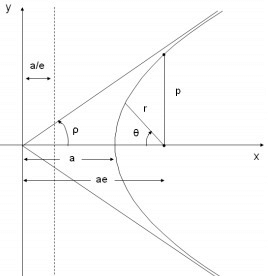
\includegraphics[width=(0.9\textwidth),height=(\textheight),keepaspectratio]{hyperbola}
\caption{Iperbole.}
\end{figure}

\begin{align*}
&\frac{x^2}{a^2}-\frac{y^2}{b^2}=1\\
&r=\frac{p}{1+e\cos{\theta}}\\
&e=\sqrt{1+\frac{b^2}{a^2}},\ p=a(e^2-1)\\
&x=a\cosh{F},\ y=b\sinh{F}
\end{align*}

\clearpage

\chapter{Equazioni differenziali}
\PartialToc

\section{Equazione di Poisson}

\subsection{Potenziale gravitazionale}

U \'e il potenziale gravitazionale, energia potenziale per unit\'a di massa.

\begin{align*}
&\nabla^2U=4\pi\rho G&\intertext{la soluzione \'e:}\\
&U(\vec{r})=-G\int\,d^3r\frac{\rho(r')}{|\vec{r}-\vec{r}'|}\\
\end{align*}

Infatti le soluzioni dell'equazione di Poisson generica \mblock{\Laplace \phi=f} si trovano a partire dalle soluzioni dell'equazione di Laplace \mblock{\Laplace\phi=0}:

\begin{align*}
&\Phi(\vec{x})=\left\{\begin{array}{c}-\frac{1}{2\pi}\log{|\vec{x}|}\ (n=2)\\
\frac{1}{n(n-2)\alpha(n)|\vec{x}|\expy{n-2}}\ (n\geq3)
\end{array}\right.&\intertext{soluzione dell'equazione di Poisson \'e}\\
&u(\vec{x})=\int_{R^n}\Phi(\vec{x}-\vec{y})f(\vec{y})\,d^ny
\end{align*}

Soluzione in 3D \'e
\begin{equation*}
\phi(\vec{x})=-\frac{1}{4\pi}\int_V\frac{f(\vec{x}'}{|\vec{x}-\vec{x}'|}\,d^3x'
\end{equation*}


\chapter{Integrali - Tecniche d'integrazione.}
\PartialToc

 
\section{Gaussian}
 
\subsection{Equazione di Saha: somma su tutti i momenti finali dell'elettrone}
\begin{align*}
&\frac{n_{r+1}}{n_r}=\frac{g_{r+1}}{g_r}\frac{8\pi}{n_eh^3}\exp{-\frac{\chi_r}{KT}}\int_0^{+\infty}p_e^2\exp{-\frac{p_e^2}{2m_eKT}}\,dp_e&\intertext{con $a^2=\frac{1}{2m_eKT}$ }\\
&\int_0^{+\infty}x^2\exp{-a^2x^2}\,dx=\frac{\sqrt{\pi}}{4a^3}
\end{align*}



\section{Step integral of Lane-Emden equation}
 
 I use the Lane-Emden eqution in the form
 \begin{equation*}
 \frac{d^2w}{dz^2}=-[\frac{2}{z}\frac{dw}{dz}]-w^n
 \end{equation*}
 
 Stepping outward in radius from the center $w_{i+1}$ is given by previous $w_i$ plus amount the density changes by over the step
 \begin{align*}
 &w_{i+1}=w_i+\Delta z(\frac{dw}{dz})_{i+1}&\intertext{the rate of changes of density with radius is unknown but I can write it in term of second derivative:}\\
 &(\frac{dw}{dz})_{i+1}=(\frac{dw}{dz})_i+\Delta z\frac{d^2w}{dz^2}&\intertext{e sostituendo l'espressione per la derivata seconda data dall'equazione di Lane-Emden ho:}\\
 &(\frac{dw}{dz})_{i+1}=(\frac{dw}{dz})_i-[\frac{2}{z_i}(\frac{dw}{dz})_i+w_i^n]\Delta z
 \end{align*}
 
 Starting at center where
 \begin{align*}
 &\frac{dw}{dz}|_0=0\\
 &w(0)=1
 \end{align*}
I determine $(\frac{dw}{dz})_{i+1}$ and then $w_{i+1}$.
 
 
\chapter{Corpi autogravitanti in equilibrio}
\PartialToc


\section{Corpi in rotazione: modello di fluido autogravitante.}
 
\subsection{McLaurin spheroids}

The shape of McLaurin spheroid is described by eccentricity
\begin{equation*}
e^2=\frac{a^2-b^2}{a^2}
\end{equation*}
where a and b are the major and minor half-axes of meridional cross-section.
 
\subsection{Accelerazione di gravit\'a}

Formule di McLaurin
\begin{align*}
&g_{eq}=2\pi G\rho a \frac{\sqrt{1-e^2}}{e^3}[\arcsin{e}-e\sqrt{1-e^2}]\\
&g_{eq}=4\pi G\rho a \frac{\sqrt{1-e^2}}{e^3}[e-\sqrt{1-e^2}\arcsin{e}]
\end{align*}

 
\chapter{Gas di Fermi degenere (elettroni)}
\PartialToc


\section{Gas di elettroni degenere per velocit\'a relativistiche}
 
\subsection{Variabili adimensionali}

\begin{align*}
\xi=\frac{p}{m_ec}\\
x=\frac{p_F}{m_ec}
\end{align*} 

\subsection{Pressione}
 
 \begin{align*}
 &P=\frac{8\pi c}{3h^3}\int_0^{p_F}p^3\frac{p/(mc)}{\sqrt{1+p^2/(mc)^2}}\,dp\\
 &=\frac{8\pi c^5m^4}{3h^3}\int_0^x\frac{\xi^4}{\sqrt{1+\xi^2}}\,d\xi\\
 &\int_0^x\frac{\xi^4}{\sqrt{1+\xi^2}}\,d\xi\\
 &=\frac{1}{8}[x(2x^2-3)\sqrt{1+x^2}+3\arcsinh{x}]
 \end{align*}
 
quindi riscrivo

\begin{align*}
&P=\frac{\pi m^4c^5}{3h^3}f(x)\\
&f(x)=[x(2x^2-3)\sqrt{1+x^2}+3\arcsinh{x}]\\
&=[x(2x^2-3)\sqrt{1+x^2}+3\ln{(x+\sqrt{1+x^2})}
\end{align*}

\subsection{Energia interna}

\begin{align*}
&U=\int_0^{p_F}f(p)E(p)\,dp=\frac{8\pi}{h^3}\int_0^{p_F}E(p)p^2\,dp&\intertext{esplicitando la dipendenza dell'energia \mblock{E=E_{T}-mc^2} ottengo}
&U=\frac{\pi m^4c^5}{3h^3}g(x)\\
&g(x)=8x^3[\sqrt{x^2+1}-1]-f(x)
\end{align*}

\section{Casi limite}

\subsection{Importance of relativistic effect: parametro x.}

\begin{align*}
&x=\frac{p_F}{mc}=\frac{v_F/c}{\sqrt{1-(v_F/c)^2}}\\
&\frac{v_F^2}{c^2}=\frac{x^2}{1+x^2}
\end{align*}

Se $x\ll1$ gli elettroni hanno velocit\'a non relativistiche; nel caso $x\gg1$ $\frac{v_F}{c}\approx1$.

\subsection{Espressioni asintotiche per $f(x)$ e $g(x)$: caso non relativistico ($x\to0$).}

\begin{align*}
&f(x)\abc{x\to0}\frac{8}{5}x^5\\
&g(x)\abc{x\to0}\frac{12}{5}x^5
\end{align*}

\subsection{Espressioni asintotiche per $f(x)$ e $g(x)$: caso ultra relativistico ($x\to\infty$).}

\begin{align*}
&f(x)\abc{x\to\infty}2x^4\\
&g(x)\abc{x\to\infty}6x^4
\end{align*}

\part{Physical Background}


\chapter{Relativity}
\PartialToc

\section{Kinematic}

\begin{align*}
&p=\frac{m_ev}{\sqrt{1-v^2/c^2}}\\
&E_{tot}=\frac{m_ec^2}{\sqrt{1-v^2/c^2}}=m_ec^2\sqrt{1+\frac{p^2}{m_e^2c^2}}\\
&E_k=\sqrt{p^2c^2+m^2c^4}-mc^2\\
&pc\ll mc^2:\ E_k\to\frac{p^2}{2m}\\
&pc\gg mc^2:\ E_k\to pc
\end{align*}


\chapter{Dynamic of fluids. MHD equations.}
\PartialToc

\section{Vectorial and upper order identity}

\begin{align*}
&\nabla\cdot(\vec{v}\cdot\ten{P})=\vec{v}\cdot(\nabla\cdot\ten{P})+\ten{P}:(\nabla\vec{v})\\
&\ten{A}:\ten{B}=\trace{A*B^T}
\end{align*}

\section{Dynamic equilibrium}

When there is motion we have a dynamical equilibrium and we have to add inertial term to hydrostatic condition (equilibrium is referred to comoving frame with fluid).

\subsection{Acceleration in fluid with spherical symmetry}

\begin{align*}
&\frac{v(r+v\,dt,t+dt)-v(r,t)}{dt}\to\TDof{t}v\\
&=\PDy{t}{v}+v\PDy{r}{v}&\intertext{Acceleration results from change in the velocity field at given place and the change due to the fact that fluid element moves. The first term is Eulerian variation, the whole is Lagrangian derivative. More generaly Lagrangian derivative defines the rate of change along with moving fluid $\downarrow$}\\
&\TDof{t}=\PDof{t}+\scap{v}{\nabla}
\end{align*}

\subsection{Eulerian description}

In Eulerian description all physical properties of fluid ($\vec{v}$, P $\rho$, T, etc) are regarded as field quantities depending on $(\vec{r},t)$ where $\vec{r}$ is the position of point of observation.

\subsection{Lagrangian description}

Motion of a given fluid element is followed: $\vec{r}$ denotes position of a given element depending on t and in general in 3D space on 3 parameter, if the are the component of the vector which was identical to $\vec{r}$ at say $t=0$ we have $\vec{r}(\vec{a},t)$ where $\vec{r}(\vec{a},0)=\vec{a}$.

Lagrangian description is used in 1D problem where a may represent T or interior mass.

\subsection{Material derivative}

Using the Lagrangian position variable we have 
\begin{align*}
&\dvec{r}=\TDy{t}{\vec{r}}=\vec{v}(\vec{r},t)\\
&\TDof{t}=\PDof{t}+\scap{v}{\nabla}
\end{align*}


\subsection{Equilibrium condition}

\begin{align*}
&\TDy{r}{P}+G\frac{m(r)\rho(r)}{r^2}=0&\intertext{alla condizione di equilibrio idrostatico aggiungo il termine dovuto all'accelerazione $\rho\TDy{t}{v}$ nel riferimento solidale all'elemento di fluido:}\\
&\rho(\PDy{t}{v}+v\PDy{r}{v})+\PDy{r}{P}+\frac{Gm(r)}{r^2}\rho=0&\intertext{vedi conservazione del momento}
\end{align*}

\subsection{Stationary flow. Bernoulli's equation: barotropic regime.}
It show how velocity of flow is affected by gravity and changes in density
\begin{align*}
&\rho(v\PDy{r}{v})+\PDy{r}{P}+\frac{Gm(r)}{r^2}\rho=0&\intertext{in stationary flow $v$ is function of r alone. In barotropic regime  $P(\rho)$ and $\uparrow$ integrates to }\\
&\frac{v^2}{2}+F(\rho)-\frac{GM}{r}=const&\intertext{$\uparrow$ Bernoulli's equation.}\\
&\rho\,dF=dP=c_s^2\,d\rho
\end{align*}

For a perfect adiabatic gas $F=\frac{\gamma}{\gamma-1}\frac{P}{\rho}$ and Bernoulli's equation become

\begin{align*}
&\frac{v^2}{2}+\frac{c_s^2}{\gamma-1}-\frac{GM}{r}=\frac{v_0^2}{2}+\frac{c_{s0}^2}{\gamma-1}-\frac{GM}{r_0}&\intertext{In the isothermal regime the sound speed is a constant:}\\
&\gamma\to1,\quad c_s^2=\TDy{\rho}{P}
\end{align*}

\section{Leggi di conservazione}

In astrophysical context $\vec{f}$ the force per unit mass is denoted by $\vec{g}$ the gravitational acceleration.

\subsection{Mass conservation}

A shell $[r,r+dr]$ contains mass $4\pi r^2\rho\,dr$: in infinitesimal time $dt$ a particle moves by $v(r,t\,dt)$ so

\begin{align*}
&r^2\to r^22rv\,dt\\
&dr\to dr+dr\PDy{r}{v}\,dt\\
&\rho\to\rho+(\PDy{t}{\rho}+v\PDy{r}{\rho})\,dt\\
\end{align*}

The total change in $r^2\rho\,dr$ must be zero
\begin{align*}
&2rv\rho+r^2(\PDy{t}{\rho}+v\PDy{r}{\rho})+r^2\rho\PDy{r}{v}=\\
&\TDy{t}{\rho}+\rho\underbrace{(\PDy{r}{v}+\frac{2v}{r})}_{\div{v}=\div{(v\frac{\vec{r}}{r})}}=0&\intertext{In general case (when no sperical symmetry is assumed)}\\
&\TDy{t}{\rho}+\rho\scap{\nabla}{v}=\PDy{t}{\rho}+\nabla\cdot(\rho\vec{v})=0&\intertext{infatti la trasformazione subita da un elemento di fluido in tempo $dt$:}\\
&\vec{r}\to\vec{r}+\vec{v}\,dt&\intertext{ \'e associata alla trasformazione nell'elemento di volume infinitesimo}\\
&dV\to\,dV(1+dt\,\scap{\nabla}{v})\quad (\frac{d\ln{dV}}{dt}=\scap{\nabla}{v})&\intertext{quindi in un fluido incompressibile the velocity is free of divergence $\div{v}=0$.}
\end{align*}

\subsubsection{Mass conservation: Eulerian and Lagrangian descriptions.}

Nella descrizione Euleriana la conservazione della massa si esprime tramite l'equazione di continuit\'a:

\begin{align*}
&\PDy{t}{\rho}+\nabla\cdot(\rho\vec{v})=0&\intertext{$\rho\vec{v}$ is the current density of mass flow}\\
&\frac{1}{\rho}\TDy{t}{\rho}=-\scap{\nabla}{v}\\
&\frac{1}{V}\TDy{t}{V}=\scap{\nabla}{v}\\
&\TDof{t}(\rho\,d\tau)=\TDof{t}(dm)=0
\end{align*}

Nella descrizione Lagrangiana \'e conveniente considerare l'espressione per la posizione di ogni elemento di massa $\vec{r}=\vec{r}(\vec{a},t)$ come una trasformazione continua di variabili (dot stands for Stokes derivative)

\begin{align*}
&\rho(\vec{a},t)J(\vec{r}[\vec{a},t])=\rho_0=\rho(\vec{a},t=0)\\
&J(\vec{r}[\vec{a},t])=|\PDy{a_k}{x_j}|,\quad\Rightarrow\quad\dot{J}\\
&=J\sum_i\PDy{a_i}{v_i}=J\scap{\nabla}{v}&\intertext{quindi, segue il risultato analogo a quello nella descrizione Euleriana:}\\
&\frac{\dot{\rho}}{\rho}=-\scap{\nabla}{v}
\end{align*}

\subsection{Momentum conservation}

Per i fluidi la conservazione della quantit\'a di moto \'e in sostanza la seconda legge di Newton: l'equazione risultante \'e l'equazione del moto. Nella descrizione Euleriana

\begin{align*}
&\rho\TDy{t}{\vec{v}}=-\nabla\cdot\ten{P}+\rho\vec{f}&\intertext{$\vec{v}$ is the fluid velocity (momentum per unit mass) and $\vec{f}$ is the total body or external force per unit mass and $\ten{P}$ is pressure tensor (symmetric for angular momentum conservation). Considero il caso di un corpo autogravitante:}\\
&\rho\TDy{t}{\vec{v}}+\nabla P+\rho\nabla U=\rho(\PDy{t}{\vec{v}}+\vec{v}\cdot\nabla\vec{v})\\
&+\nabla P+\rho\nabla U=0&\intertext{U is the gravitational potential energy per unit mass. Without $\rho\nabla U$ $\uparrow$ \'e l'equazione di Eulero.}
\end{align*}

The equation of motion may also be written in a form that doesn't require mass conservation
\begin{align*}
&\PDy{t}{(\rho\vec{v})}+\nabla\cdot\underbrace{(\rho\vec{v}\vec{v}+\ten{P})}_{\parbox{1cm}{Momentum flux density}}=\rho\vec{f}&\intertext{In absence of external force the rate of decreases of momentum (of volume density $\rho\vec{v}$) in a fixed volume of the fluid is equal to net outward rate of flow of momentum of flux $(\rho\vec{v}\vec{v}+\ten{P})\cdot\hat{n}$.}
\end{align*}

If stresses reduce to pure hydrostatic pressure $\ten{P}=P*Id$: the force due to stresses acting on a surface $dS\hat{n}$ is $-P\hat{n}\,dS$ that is a force acting along inward normal

\begin{align*}
&\rho\TDy{t}{\vec{v}}=-\nabla P+\rho\vec{f}&\intertext{$\uparrow$ is assumed mass conservation.}\\
&\nabla P=\rho\vec{f}&\intertext{$\uparrow$ hydrostatic equilibrium in a static fluid $\vec{v}=0$.}\\
&\PDy{t}{(\rho\vec{v})}+\nabla\cdot(\rho\vec{v}\vec{v}+PI)=\rho\vec{f}&\intertext{$\uparrow$  mass conservation is NOT assumed.}
\end{align*}

When turbolence, viscosity or large-scale magnetic field are present their effects can be described in terms of a pressure tensor.

\subsection{Energy conservation}

\subsubsection{Mechanical energy}

\begin{align*}
&\TDof{t}(\frac{1}{2}v^2)=-\frac{1}{\rho}\vec{v}\cdot(\nabla\cdot\ten{P})+\scap{f}{v}&\intu{say that the rate of increse of the kinetic energy per unit mass is equal to the rate at which the pressure gradient and body forces are doing work on the unit mass. It's obtained from momentum equation in Eulerian form $\downarrow$ diveded by $\rho$ and reduced to scalar multiplying both sides by $\vec{v}$}\\
&\rho\TDy{t}{\vec{v}}=-\nabla\cdot\ten{P}+\rho\vec{f}
\end{align*}

We have an integral form: supposing $\vec{v}\cdot\ten{P}\cdot\,d\vec{S}$ is small ($\ten{P}$ small near the surface or ($\vec{v}\cdot\ten{P}$) is nearly perpendicular to $d\vec{S}$ as in steadly rotating star) and stresses reduce to pure pressure (and using mass conservation)
\begin{align*}
&\TDof{t}\int_M\frac{1}{2}v^2\,dm\\
&=\int_M[P\TDof{t}(\frac{1}{\rho})]\,dm+\int_M\scap{f}{v}\,fm&\intertext{the first integral on the right side of $\uparrow$ is sum over all mass elements in entire system of the rate of \mblock{P\,dV(V=\frac{1}{\rho})} work that the material in each such mass element is doing on its surroundings.}
\end{align*}

\subsubsection{Thermal and Mechanical energy}

Conservation of thermal and mechanical energy gives the rate of change of kinetic and internal energy of a unit mass of fluid as it moves about.

Sia E l'energia interna, $\vec{f}$ la risultante delle forze esterne, e $\TDy{t}{q}$ il bilancio di calore lungo la linea di flusso, tutti per unit\'a di massa: uso il princio di conservazione della massa.

\begin{align*}
&\TDof{t}(\frac{1}{2}v^2+E)=-\frac{1}{\rho}\nabla\cdot(\ten{P}\cdot\vec{v})+\scap{f}{v}+\TDy{t}{q}&\intertext{l'equazione di Bernulli \'e un caso particolare di $\uparrow$.}
\end{align*}

Se non uso la conservazione della massa
\begin{align*}
&\PDof{t}(\rho E+\frac{1}{2}\rho v^2)\\
&+\nabla\cdot(\rho E\vec{v}+\frac{1}{2}\rho v^2\vec{v}+\ten{P}\cdot\vec{v})=\\
&=\rho\scap{f}{v}+\rho\TDy{t}{q}\\
\end{align*}

The quantity in parentheses is the energy flux vector
\begin{equation*}
\vec{j}_E=(\rho E\vec{v}+\frac{1}{2}\rho v^2\vec{v}+\ten{P}\cdot\vec{v})
\end{equation*}
\index{energy flux vector}
since in absence of external forces $\vec{f}=0$ and of heat gains or losses $\TDy{t}{q}=0$ the rate of decreses of sum of internal and kinetic energy (of volume density $\rho E+\frac{1}{2}\rho v^2$) in a fixed volume is equal to total outward rate of flux of energy across the surface bounding fixed volume $\oint_S\,d\vec{S}=\vec{j}_E$. If stresses reduce to hydrostatic pressure
\begin{align*}
&\vec{j}_E=\rho\vec{v}(\frac{1}{2}v^2+E+\frac{P}{\rho})&\intertext{$E+\frac{P}{\rho}$ is the enthalpy per unit mass.}
\end{align*}

\subsubsection{Thermal energy alone}

Generalized form of first principle of TD: dalla conservazione dell'energia meccanica e della somma dell'energia meccanica e termica segue
\begin{align*}
&\TDy{t}{E}=-\frac{1}{\rho}\ten{P}:(\nabla\vec{v})+\TDy{t}{q}&\intertext{if stresses reduce to pure pressures:}\\
&\TDy{t}{q}=\TDy{t}{E}+P\TDof{t}(\frac{1}{\rho})=\TDy{t}{E}+P\TDy{t}{V}\label{eq:Eintconservation}
\end{align*}

\subsection{Internal Energy conservation, constant composition, equation of states and adibatic exponent}

For astrophysical purpose 3 equivalent form of internal energy conservation are useful. The adiabatic exponents measure the response of system to adiabatic changes

Con le ipotesi aggiuntive che la composizione chimica sia costante, che la pressione sia determinata da una funzione di stato determinata da una coppia di variabili termodinamiche tipo $P(\rho,T)$ e analogamente per energia interna $E(\rho,T)$:

\begin{align*}
&\TDy{t}{\ln{P}}=\Gamma_1\TDy{t}{\ln{\rho}}+\frac{\rho(\Gamma_3-1)}{P}\TDy{t}{q}\\
&(=\Gamma_1\TDy{t}{\ln{\rho}}+\frac{\chi_T}{c_VT}\TDy{t}{q})\\
&\TDy{t}{\ln{T}}=(\Gamma_3-1)\TDy{t}{\ln{\rho}}+\frac{1}{c_VT}\TDy{t}{q}\\
&\TDy{t}{\ln{T}}=\frac{\Gamma_2-1}{\Gamma_2}\TDy{t}{\ln{P}}+\frac{1}{c_PT}\TDy{t}{q}&\intertext{$c_V$ e $c_P$ sono i colari specivici per unit\'a di massa, }\\
&\chi_T=(\PDly{T}{P})_{\rho},\quad \chi_{\rho}=(\PDly{\rho}{P})_{T}&\intertext{gli esponenti adiabatici}\\
&\Gamma_1=(\TDly{\rho}{P})_{Ad},\ \Gamma_3-1=(\TDly{\rho}{T})_{Ad},\\ &\frac{\Gamma_2-1}{\Gamma_2}=(\TDly{P}{T})_{Ad}=\frac{\Gamma_3-1}{\Gamma_1}&\intertext{da cui seguono le relazioni:}\\
&\Gamma_1=\chi_{\rho}+\chi_T(\Gamma_3-1),\\ &\gamma=\frac{c_P}{c_V}=\frac{\Gamma_1}{\chi_{\rho}},\ \Gamma_3-1=\frac{P\chi_T}{\rho c_VT}&\intertext{la terza di $\uparrow$ \' equivalente alla cos\'i detta relazione di reciprocit\'a}\\
&(\PDly{\rho}{E})_T=\frac{P}{\rho E}(1-\chi_T)&\intertext{Vedi Landau statistical Physics intorno al $\S16$.}
\end{align*}

La condizione che la pressione sia definita dalla funzione termodinamica equivale a trascurare la viscosit\'a radiativa e molecolare, i campi magnetici su larga scala e le turbolenze.


\section{Transport}

\subsection{scalar quantity}

The mean free path of a particle is $l_c$: if Q depends only on z we consider two surfaces at $z-\frac{l_c}{2}$ and $z+\frac{l_c}{2}$.

\begin{align*}
&Q(z+\frac{l_c}{2})-Q(z-\frac{l_c}{2})\approx l_c\PDy{z}{Q}&\intu{net quantity of Q transfered (collisional processes), and vice versa.}\\
&F_Q=nv_T[Q(z-\frac{l_c}{2})-Q(z+\frac{l_c}{2})]\\
&\approx-nv_Tl_c\PDy{z}{Q}\\
&\vec{F}_Q=-nv_Tl_c\nabla Q&\intu{$l_c$ gives order of magnitude: precise numerical coefficient have to take in account for velocity distribution.}\\
&\TDof{t}\int_V\,dVQ=-\int_S\,dS\scap{n}{F_Q}\\
&=-\int_V\,dV\scap{\nabla}{F}_Q&\intu{no sources in the volume}\\
&\rho\TDy{t}{Q}=\nabla\cdot(\rho v_Tl_C\nabla Q)&\intertext{mass is conserved so Lagrangian derivative of $\rho\,dV$ vanishes.}
\end{align*}

\subsection{Heat}

\begin{align*}
&Q=c_PT&\intu{thermal energy per unit mass}\\
&\chi=v_Tl_C&\intu{heat flows to the cooler parts: heat transport coefficient or heat diffusivity}\\
&\rho\TDy{t}{Q}=\nabla\cdot(\rho\chi\nabla (c_PT))+S&\intu{heat transport equation S is a source or sink: production rate per unit volume}\\
&\rho c_P\TDy{t}{T}=\kappa \nabla^2T+S&\intu{$\kappa=\rho\chi c_P$, $\rho$, $\chi$, $c_P$ are constant.}\\
\end{align*}

The heat transport equation  must be supplemented with boundary conditions at surface (radiative loss) and continuity condition across sharp transition (in planets: core mantle): with energy source at the transition (with dimension of flux) we expect a jump in the flux $\rho\chi\hat{n}\cdot\nabla(c_PT)$ so $\mvar{}[\rho\chi\hat{n}\cdot\nabla(c_PT)]=F$.

If $T(z,t)$ is the only variable and fluid is at rest
\begin{align*}
&\PDy{t}{T}=\chi\PtwoDy{z}{T}&\intu{parabolic equation. An initial spike spreads after time t over distance $\sqrt{\chi t}$ and there is no wave propagation}\\
&T(z,t)=\frac{K}{2\sqrt{\pi\chi t}}\exp{-\frac{z^2}{4\chi t}}\\
&\lim_{t\to0}T(z,t)=K\delta(z)&\intertext{total thermal energy is conserved $\propto\int\,dz T=K$}
\end{align*}

\subsection{Momentum: viscosity.}

\begin{align*}
&Q=m_{mol}v_x(z)&\intertext{the sheared velocity field is smoothed out}\\
&\eta=\rho v_Tl_C&\intu{viscosity coefficient}\\
&\rho(\PDy{t}{\vec{v}}+\vec{v}\cdot\nabla\vec{v})+\nabla P+\rho\nabla U\\
&=\eta[\nabla^2\vec{v}+\frac{1}{3}\nabla(\scap{\nabla}{v})]&\intd{for incompressible flow $\scap{\nabla}{v}=0$ becomes}\\
&\rho(\PDy{t}{\vec{v}}+\vec{v}\cdot\nabla\vec{v})+\nabla P+\rho\nabla U=\eta\nabla^2\vec{v}&\intu{Navier-Stokes equation, $\eta/\rho$ is the kinematic viscosity.}
\end{align*}

Viscosity results in dissipation, the kinetic energy of the fluid motion is transformed into heat and should be accounted for in heat transfer equation
\begin{align*}
&E{Kin}=\frac{1}{2}\int\,dV\rho v^2\\
&\TDy{t}{E{Kin}}=-\frac{1}{2}\int\,dVq_{ij}(\PDy{r_j}{v_i}+\PDy{r_i}{v_j})&\intertext{$q_{ij}$ is the viscous stress tensor depending on velocity and its derivatives respect spatial coordinates}\\
&\TDy{t}{E{Kin}}=-\frac{\eta}{2}\int\,dV(\PDy{r_j}{v_i}+\PDy{r_i}{v_j})^2
\end{align*}

The relevance of viscosity is described by Reynold number\index{Reynold number} 
\begin{align*}
Re=\frac{\rho Lv}{\eta}&\intertext{L is a macroscopic characteristic length, v is a typical velocity of the flow}
\end{align*}


\section{Partially/totally ionized gas.}

At sufficient high temperatures and low densities (possibly under strong UV radiation from the sun) the gas may becomes partially or totally ionized. When the number of particles in square cube $\lambda_D$ is large and for scales larger than $\lambda_D$ approximate charge neutrality holds and we can describe the gas as a single neutral fluid.

Relative motions of electrons and ions produce electric currents and magnetic fields.

Astrophysical fluids are at least partially ionized  thus electromagnetic forces can be more important for macroscopic dynamics: Magneto-hydrodynamics is the name used when we deal with continuum mechanics for charged matter otherwise plasma physics.

\section{Maxwell's equations}

At microscopic level the field $\vec{E},\vec{B}$ are determined by charge densities $\sigma_c$ and current densities $\vec{J}$
\begin{align*}
&\scap{\nabla}{E}=4\pi\rho_c\\
&\vecp{\nabla}{B}-\frac{1}{c}\PDy{t}{\vec{E}}=\frac{4\pi}{c}\vec{J}&\intertext{Gaussian Units}
\end{align*}

and Faraday's law, absence of magnetic monopoles

\begin{align*}
&\vecp{\nabla}{B}+\frac{1}{c}\PDy{t}{\vec{B}}=0\\
&\scap{\nabla}{B}=0
\end{align*}

An arbitrary EM field tha fulfils the continuity equation
\begin{equation*}
\PDy{t}{\rho_c}+\scap{\nabla}{J}=0
\end{equation*}
can be propagated in time.

At macroscopic level in presence of matter the electric field is affected also by polarization and similarly magnetic fields
\begin{align*}
&\scap{\nabla}{D}=4\pi\rho_c\\
&\vecp{\nabla}{H}-\frac{1}{c}\PDy{t}{\vec{D}}=\frac{4\pi}{c}\vec{J}\\
&\vecp{\nabla}{B}+\frac{1}{c}\PDy{t}{\vec{B}}=0\\
&\scap{\nabla}{B}=0&\intertext{Gaussian Units}
\end{align*}

We need constitutive relations between $\vec{B}$, $\vec{H}$ and $\vec{E}$, $\vec{D}$: when fields are weak and matter isotropic
\begin{align*}
&\vec{B}=\mu\vec{H}\\
&\vec{D}=\epsilon\vec{E}
\end{align*}
In normal modes of oscillation the electric and magnetic response depends on the mode: the constitutive equations are expressed in term of Fourier component of the field.

\section{Magneto-hydrodynamics}

\subsection{Equation for boh fluid}

The equation of motion (confronta con cox, bertotti, Dalsgaard\index{da fare: eq moto})

\begin{align*}
&\rho\PDy{t}{\vec{v}}+\nabla P+\rho\nabla U\\
&=\rho(\PDy{t}{\vec{v}}+\scap{v}{\nabla\vec{v}})+\nabla P+\rho\nabla U=0&\intertext{without the term $\rho\nabla U$ is called the Euler equation}
\end{align*}

\subsection{Electrically conductive fluid}

In a moving conductor Ohm's law must be modified
\begin{align*}
&\vec{J}=\sigma(\vec{E}+\frac{1}{c}\vecp{v}{B})&\intertext{In presence of factor that destroy the isotropy of the fluid the conductivity is a tensor. When the conductivity is large enough that we can replace the equation $\uparrow$ with:}\\
&\vec{E}+\frac{1}{c}\vecp{v}{B}=0
\end{align*}

In electrically conductive fluid the magnetic force must be added to EOM. A charge q moving with velocity $\vec{u}$ in a magnetic field $\vec{B}$ suffers a Lorentz force $\frac{q}{c}\vecp{u}{B}$: for all charged particles in an infinitesimal volume we get $\sum q\vecp{u}{B}=\vecp{J}{B}\,dV$. Aggiungo il contributo della forza di Lorentz per unit\'a di volume all'equazione di conservazione della quantit\'a di moto:
\begin{equation*}
\rho\TDy{t}{\vec{v}}+\nabla P+\rho\nabla U=\frac{1}{c}\vecp{J}{B}
\end{equation*}

La pressione deve essere espressa in funzione della densit\'a o direttamente tramite una dipendenza politropica o indirettamente tramite l'equazione di stato e del bilancio energetico.

Since electric and magnetic fields are created by motions of fluid at speed $v\ll c$: their time and space variations are related by \mblock{\PDof{t}\approx v\nabla\ll c\nabla} and we have the Ampere law in simpler form neglecting displacement current
\begin{align*}
&c\vecp{\nabla}{B}=4\pi\vec{J}&\intertext{$\uparrow$ current density is solenoidal and net charges are neglected. This is in agreement with general property of plasma in which there are no charge fluctuations in volumes much larger than $\lambda_D$. The small charge density can be recovered taking the divergence of Ohm's law $\downarrow$}\\
&\vec{J}=\sigma(\vec{E}+\frac{1}{c}\vecp{v}{B})
\end{align*}

This approcimation cannot deal with electromagnetic waves for wich E and B are of same order of magnitude.

\subsection{Magnetic stress tensor}

Scrivo la forza magnetica per unit\'a di volume

\begin{align*}
&\vec{f}=\frac{1}{c}\vecp{J}{B}+\div{-\frac{B^2}{8\pi}\ten{1}+\frac{\ten{B}}{4\pi}}\\
&=\div{\ten{{P^M}}}&\intertext{$\uparrow$ ho usato espressione}\\
&(\nabla\wedge\vec{B})\wedge\vec{B}
\end{align*}
\index{(C) espressione magnetic stress tensor}
Let's illustrate the signifiance of magnetic stress tensor with two examples:

\begin{itemize*}
\item Magnetic field along z but with arbitrary intensity $B(x,y)$.

$\ten{{P^M}}$ is a scalar and a flow in $(x,y)$ plane is governed by total pressure

\begin{align*}
&P+\frac{B^2}{8\pi}&\intertext{where the latter term $\frac{B^2}{8\pi}$ is the magnetic pressure that has the effect of pushing the flow away from high intensity regions.}
\end{align*}

This happens , ie, in the interaction between supersonic solar wind and Earth's dipole field which acts like an obstacle with the magnetic pressure giving rise to a shock front.

The magnetic pressure prevail over the fluid pressure P when the ratio $\beta=\frac{8\pi P}{B^2}$ is small.

\item B has uniform intensity but its direction $\hat{n}$ is not.

Only potive component along $\hat{n}\hat{n}$ is relevant

Transversal waves with Alfv\'en speed 

\begin{align*}
&V_A=\sqrt{\frac{B^2}{4\pi\rho}}
\end{align*}

\end{itemize*}

\section{The induction equation. Magnetic diffusion coefficient}

\subsection{Induction equation}

When conductivity $\sigma$ is constant
\begin{align*}
&\PDy{t}{\vec{B}}=\nabla\wedge(\vec{v}\wedge\vec{B})+\frac{c^2}{4\pi\sigma}\nabla^2\vec{B}\\
&\lambda=\frac{c^2}{4\pi\sigma}&\intertext{$\uparrow$ is the magnetic diffusion coefficient. The analog of viscosity. In a medium at rest ($\vec{v}=0$) the induction equation is equivalent to heat equation with conductivity $\lambda$: an initial magnetic field spike after a time t spread over a distance $c\sqrt{\lambda t}$.}
\end{align*}
 
\subsection{Infinite conductivity limit}

In a perfectly conductive fluid holds
\begin{align*}
&\vec{E}+\frac{1}{c}\vec{v}\wedge\vec{B}=0&\intertext{contrary to Newtonian dynamics in this case the electromagnetic field determines the component of the velocity orthogonal to the line of force not its time derivative}\\
&\vec{v}_{\perp}=c\frac{\vecp{E}{B}}{B^2}
\end{align*}
La componente lungo $\vec{B}$ della velocit\'a obbedisce all'equazione della conservazione dell'impulso. Dalla legge di Ohm risulta che il campo elettrico e magnetico sono ortogonali, il campo elettrico lungo le linee di forza \'e annullato dal moto delle cariche. 

\subsection{MHD equation: infinite conductivity, no gravity, no viscosity.}

\begin{align*}
&\rho[\PDy{t}{\vec{v}}+(\scap{v}{\nabla})\vec{v}]+\nabla P=\frac{1}{4\pi}(\nabla\wedge\vec{B})\wedge\vec{B}\\
&\PDy{t}{\rho}+\nabla\cdot(\rho\vec{v})=0\\
&\PDy{t}{\vec{B}}=\nabla\wedge(\vec{v}\wedge\vec{B})
\end{align*}


\section{Conservation of magnetism and vorticity (???).}

\subsection{Rate changes surface dragged along flux}

\begin{align*}
&\TDof{t}(d\vec{r})=(d\vec{r}\cdot\nabla)\vec{v}\\
&\TDof{t}(dS_i)=dS_i\scap{\nabla}{v}-dS_j\PDy{r^i}{v^j}\\
&dV=d\vec{S}\cdot\,d\vec{r}=\frac{dm}{\rho}
\end{align*}

\subsection{Conservation magnetic flux and circulation}

\begin{align*}
&\TDy{t}{\vec{B}}=\PDy{t}{\vec{B}}+(\scap{v}{\nabla})\vec{B}\\
&=(\scap{v}{\nabla})\vec{v}-\vec{B}(\scap{\nabla}{v})+\frac{c^2}{4\pi\sigma}\nabla^2\vec{B}&\intu{Lagrangian change in magnetic field}\\
&\TDof{t}(\vec{B}\cdot\,d\vec{S})=\frac{c^2}{4\pi\sigma}\,d\vec{S}\cdot\nabla^2\vec{B}&\intu{Lagrangian change in magnetic flux through $d\vec{S}$}
\end{align*}

\subsection{Frozen flux and freezing theorem}

When conductivity is infinite the flux through a surface attached to the fluid is constant and dragged along with the fluid (Alfv\'en's frozen flux theorem). In the collapse of a cosmic body of size R, B increases as $1/R^2$: this can produces large amplification of magnetic field. Similarly when a charged particle moves in a slowly varying magnetic field the flux embraced in a Larmor gyration remains almost constant.

Freezing theorem (cosmic physics/solar wind)
\begin{align*}
&\TDof{t}(d\vecp{r}{B})=-\vec{B}\wedge(\,d\scap{r}{\nabla})\vec{v}+\\
&+\,d\vec{r}\wedge[(\scap{B}{\nabla})\vec{v}-\vec{B}(\scap{\nabla}{v})]\\
&+\frac{c^2}{4\pi\sigma}\,d\vec{r}\wedge\nabla^2\vec{B}&\intertext{If initially $\vec{r}$ and $\vec{r}+d\vec{r}$ lie on same line of force so that $d\vecp{r}{B}=0$ ($d\vec{r}$ and $\vec{B}$ being parallel) then the first two terms on rhs of $\uparrow$ cancel each other.}
\end{align*}

In infinitely conductive plasma the condition $d\vecp{r}{B}=0$ holds forever: a line of force is tied to the fluid element lying on it.

\subsection{Kelvin vorticity theorem}
Negligible viscosity

\begin{align*}
&\TDof{t}\int_s\,d\vec{S}\cdot(\vecp{\nabla}{v})=0
\end{align*}

In a barotropic inviscid fluid the vorticity lines are anchored to the matter.


\chapter{Gravitational field}\label{chap:gravity}
\PartialToc

\section{Gravitational energy}

\subsection{Poisson's equation: superposition principle.}

$U$, energia potenziale gravitazionale per unit\'a di massa o potenziale gravitazionale, \'e soluzione dell'equazione di Poisson
\begin{equation*}
\nabla^2U=4\pi G\rho
\end{equation*}
quindi 
\begin{align*}
U(\vec{r})=-G\int d^3r'\frac{\rho(\vec{r}')}{|\vec{r}-\vec{r}'|}
\end{align*}

For a point mass M we have the monopole $U=-G\frac{M}{r}$. The linearity of poisson's equation ensure the superposition principle: the potential of N bodies is the sum of individual potentials.

\subsection{Gravitational acceleration}

We obtain the force per unit mass acting on the fluid from gravitational potential

\begin{align*}
&\vec{f}(\vec{r},t)=\vec{g}(\vec{r},t)=-\nabla U(\vec{r},t)\\
&\scap{\nabla}{f}=-4\pi G\rho
\end{align*}

\subsection{Energia gravitazionale.}
Considero massa unitaria a distanza r: l'energia potenziale dovuta a $m(r)$ \'e $-\frac{Gm(r)}{r}$. L'energia potenziale $E_g$ \'e la somma su tutti gli elementi $dm$ della stella e $-E_g>0$ \'e l'energia necessaria per espandere tutti i gusci a infinito. 

\begin{align*}
&E_g=-\int_0^M\frac{Gm(r)}{r}\,dm
\end{align*}

\section{Gravitional equilibrium}

L'equilibrio di una struttura su scala cosmica \'e determinato dall'equilibrio tra attrazione gravitazionale e pressione interna. La pressione interna \'e determinata dall ostato della materia, dalla composizione, il flusso di calore, il campo magetico, etc.

This factors are influenced by the way the body was formed and its history. Their determination require laws of microscopical physics: state of stress (pressure tensor) provides link between microscopical state and global structure. If as in fluids microscopic states have no privileged direction the pressure tensor depend only on the scalar pressure: deviation from spherical equilibrium will occur also if part of the body is solid capable of supporting tangential forces at its surface.

\section{Configurazione sferica}

\subsection{Gauss theorem}

The gravitational acceleration $\vec{g}$ produced by point mass $m$ is formally obtained from electrostatic field produced by charge $q$ substituting $q$ with $-Gm$.
\begin{align*}
&g(r)=G\frac{M(r)}{r^2}\\
&\int_S\,dS\scap{n}{g}=-4\pi GM(r)
\end{align*}

\subsection{Gravitational potential energy per unit of mass}

\begin{align*}
&\vec{g}=-\nabla U&\intertext{U is the gravitational potential energy per unit mass. Outside the mass:}\\
&U(r>R)=-\frac{GM}{r}\\
&U(r<R)=-G[4\pi\int_r^R\,drr\rho(r)+\frac{m(r)}{r}]&\intertext{$\uparrow$ inside a thin spherical shell of mass $dM$ the gravitational pull is $0$ so $U$ is constant and equal to its value just outside, \mblock{-g\frac{dM}{r}=-4\pi G\rho(r)r\,dr}, therefore the total value is the sum of shell outside r and those inside, $-G\frac{m(r)}{r}$.}
\end{align*}

\subsection{Gravitational binding energy}

\begin{align*}
&E_B=-\frac{1}{2}G\iint\frac{dm(\vec{r})dm(\vec{r'})}{|\vec{r}-\vec{r'}|}\\
&=2\pi\int_0^Rdr\,r^2\rho(r)U(r)
\end{align*}

\section{Deviazioni da simmetria sferica}

\subsection{Rotational deformations: Parametro di Helmert}

\begin{align*}
\mu_c=\frac{R^3\omega^2}{GM}&\intertext{$\uparrow$ ratio between rotational energy and gravitational binding energy: il parametro di Helmert.}
\end{align*}

\subsection{Oblateness}

Sulla superficie la deformazione \'e misurata dall'XXX

\begin{align*}
\epsilon=\frac{R_e-R_p}{R}\approx\mu_c
\end{align*}



\chapter{Statistical physics. Thermodynamics.}
\PartialToc


\section{Distribution functions}

The distribution function for a species of particle measures the density of that species in combined 6D phase space.

\subsection{Thermodynamical description is complete?}
In a rarefied medium we must question if the flow can be completely described with mean quantities $\rho$, $\vec{v}$, T (eventually $\vec{B}$).

\subsection{Thermodynamical equilibrium}

After few collision fluid is described by locally Maxwellian distribution function which depends on space and time only through n, $\vec{v}$, T
\begin{equation*}
f=n(\frac{m}{2\pi kT})\expy{\frac{3}{2}}\exp{-\frac{m|\vec{u}-\vec{v}|^2}{2kT}}
\end{equation*}

Collision occur at rate $\nu_c=n\exv{u\sigma_c}$ (collision frequency)\index{collision frequency} averaging cross sections with velocity distributions. The gas is brought into a local thermodynamical equilibrium and is described by a fluid model. Conservation laws provide time evolution for averaged quantities. After this if the system closed and isolated on space scale L and time scale $\frac{L^2}{v_Tl_c}$ it will be brought into uniform state ~\ref{eq:uniformstate} by diffusion and dissipative processes. For lo0cal thermodynamical equilibrium typical scales for macroscopic variation in time and space by external agents must be much larger than $\frac{1}{\nu_c}$ and mean free path $l_c=\frac{v_T}{\nu_c}$ resp.

\section{Thermodynamical potential}

\subsection{Funzione termica: entalpia.}

\begin{equation*}
H=E+PV
\end{equation*}

\subsection{Entropia}

\begin{align*}
ds=\frac{dq}{T}=\frac{1}{T}[(\PDy{v}{u})_T+P]\,dv+\frac{1}{T}(\PDy{T}{u})_v\,dT
\end{align*}

\subsection{Energia libera F.}

Il lavoro corrispondente ad una variazione isotermica reversibile infinitesima dello stato del corpo si pu\'o scrivere come differenziale di una certa grandezza $F$

\begin{align*}
&dU-dQ=dU-T\,dS=d(U-TS)\\
&dF=dU-T\,dS-S\,dT\\
&dq=T\,dS=dU+P\,dV\\
&dF=-S\,dT-P\,dV
\end{align*}

\subsection{Potenziale termodinamico G}

\begin{align*}
&dG=dF+P\,dV+V\,dP\\
&dG=-S\,dT+V\,dP
\end{align*}

\subsection{Dipendenza delle grandezze termodinamiche dal numero di particelle}

\begin{align*}
&U=Nf(\frac{S}{N},\frac{V}{N})\\
&F=Nf(\frac{V}{N},T)\\
&H=Nf(\frac{S}{N},P)\\
&G(=\Phi)=Nf(P,T)\\
&dH=T\,dS+V\,dP+\mu\,dN\\
&dF=-S\,dT-P\,dV+\mu\,dN\\
&dG(=d\Phi)=-S\,dT+V\,dP+\mu\,dN\\
&\mu=\Dcvar{\PDy{N}{H}}{S,P}=\Dcvar{\PDy{N}{F}}{T,V}=\Dcvar{\PDy{N}{\Phi}}{P,T}
\end{align*}

Introduco la densit\'a numerica (specifica) $N_i=\frac{n_i}{\rho}$ (particelle per grammi): lagrangian version of $n_i$ (remain constant if volume changes).

\begin{definition}{Potenziale chimico}
Il potenziale chimico \'e definito da
\begin{equation*}
\mu_i=\Dcvar{\PDy{N_1}{E}}{S,V}
\end{equation*}
Not to be confused with molecular weight.
\end{definition}

Thermodynamical equilibrium requires \mblock{\sum_i\mu_i\,dN_i=0}.

Given $(T,\rho)$ and the possible reactions we are able to find all $N_i$ for a gas in thermodynamical equilibrium: informations about $N_i$ is contained in $\mu_i$ for given $(T,\rho)$.

\subsection{Occupation number for perfect gas.}

Distribution function for the species
\begin{align*}
&n(p)=\frac{1}{h^3}\sum_j\frac{g_j}{\expp{(\frac{-\mu+E_j+E(p)}{kT})}\pm1}
\end{align*}
$\mu$ \'e il potenziale chimico delle varie specie, $j$ conta i possibili livelli energetici della specie, $g_j$ \'e la degenerazione del livello dello stato $j$, $E(p)$ \'e l'energia cinetica.

\begin{usefull}{Distribution function}
The distribution function $n(p)$ is in unit of: Particle per $(cm * \text{unit of momentum})^3$.

\end{usefull}


\subsection{Particles: Maxwell distro}

Collisions have time and space to produce local thermal Boltzmann distribution of velocities. Maxwellian distribution f in velocity space

\begin{usefull}{Maxwell distribution}

\begin{align}\label{eq:uniformstate}
&f=n(\frac{m}{2\pi kT})\expy{\frac{3}{2}}\exp{-\frac{mu^2}{2kT}}&\intertext{$f\,d^3r\,d^3u$ is the number of particles in the phase space volume element $d^3r\,d^3u$, $n=N/V$ is the number density}
\end{align}

\end{usefull}

\begin{usefull}{MB: most probable velocity. Averaged quantities}

\begin{align*}
&\TDy{v}{f}=0\\
&v_{prob.}=\sqrt{\frac{2kT}{m}}
\end{align*}

\begin{align*}
&n(\vec{r},t)=\int d^3u\,f(\vec{r},\vec{u},t)\\
&n(\vec{r},t)\vec{v}(\vec{r},t)=\int d^3u\,\vec{u}f(\vec{r},\vec{u},t)\\
&3n(\vec{r},t)kT(\vec{r},t)=m\int d^3u\,u^2f(\vec{r},\vec{u},t)\\
&=mnv_T^2\\
&v_T=\sqrt{\frac{kT}{3m}}&\intu{thermal speed}
\end{align*}

\end{usefull}



\subsection{Radiation: Planck distro}

The frenquency distribution is uniquely determined by temperature in terms of Plank's distribution function

\begin{align*}
&n_{\nu}\,d\nu\,dV=\frac{8\pi\nu^2}{c^3}\frac{d\nu\,dV}{\exp{\frac{h\nu}{kT}}-1}\\
&u_{\nu}=h\nu n_{\nu}&\intu{spectral energy density}\\
&u_{\nu}\propto\nu^2&\intu{for frequency much less than $kT/h$, that is in the Rayleigh limit:}\\
&u_{\nu}=\frac{8\pi kT}{c^3}\nu^2&\intu{Rayleigh-Jeans law.}\\
&\lambda_{Max}=\frac{b}{T},\quad b\approx0.290\si{\cm\kelvin}&\intu{Wien displacement law: wavelength at which spectral energy density has maximum.}\\
&u=\intzi\,d\nu u_{\nu}=aT^4&\intu{is finite}\\
&a=\frac{4\sigma}{c}\approx\num{7.56e-15}\si{\erg\per\cubic\cm\per\kelvin\tothe{4}}
\end{align*}


\section{Boltzmann's equation}

\subsection{Need for a closure relation}

From conservation equations we have 5 five lin. indip. relations (momentum: vectorial, energy: scalar, mass: scalar) and thirteen variables \mblock{\rho,\ u_i,\ P,\ \pi_{ik}\,(5)}.

Until we introduce a way to derive a closed set of moment equations everything has no real physical content.

\subsubsection{When we can find usefull closure relations?}

\begin{itemize}
\item Mean free path smaller than system scale length: \mblock{l\ll L}. we expect LTE for translational degrees of freedom to hold. The Chapman-Enskog procedure allow us to derive closure relations.

To zeroth-order in a systematic expansion for small $\frac{l}{L}$ we shall find that eight needed relations take the form \mblock{\pi_{ik}\approx0,\ F_i\approx0}: the neglect of diffusive effects leads to a complete set of fluid relations called Euler equations. The next order approximation are the Navier-Stokes equations in which diffusive terms \mblock{\pi_{ik},\ F_i} are not zero.

\item Mean free path much larger than system scale length, $l\gg L$: is the analogous of an optical thin system for radiative transfer but we cannot assume particle travel in straight lines because they are subjected to macroscopical large-scale forces that bend trajectories.

When collision are unimportant we have free-molecular flow (Knudsen regime) in which particles move indipendently of each others. When none of these two extreme approximations hold we study the deviations from Maxwell's distribution: a dynamical description in phase space must be adopted using differential equation for for particle distribution function f, the Boltzmann's equation.

\end{itemize}

\subsection{Higher order velocity moments of Boltzmann's equation}

Succesive approximation to the solution of Boltzmann's equation
\begin{align*}
&S=-k\int f\ln{f}\,d^3x\,d^3p&\intu{entropy of a thermally isolated gas}\\
&\begin{pmatrix}
\rho\\\rho\vec{u}\\\rho U\\
\end{pmatrix}
=\int\begin{pmatrix}
m\\m\vec{v}\\\frac{m}{2}|\vec{v}-\vec{u}|^2\\
\end{pmatrix}f(\vec{x},\vec{v},t)\,d^3v\\
&\PDy{t}{f}+\vec{v}\cdot\PDy{\vec{x}}{f}+\dvec{p}\cdot\PDy{\vec{p}}{f}=C(f)=\Dcvar{\frac{\delta f}{\delta t}}{coll}\\
&\Dcvar{\frac{\delta f}{\delta t}}{coll}=\int|\vec{v}-\vec{v}_2|\sigma(\Omega)*\\
&*[f(\vec{v}')f(\vec{v}_2')-f(\vec{v})f(\vec{v}_2)]\,d\Omega\,d^3v_2&\intu{Boltzmann's equation: we wish to derive equations governing spacetime evolution of $\rho$, $\vec{u}$, $U$. We multiply BE by \mblock{\chi(\vec{v}=\insieme{m,m\vec{v},m\vec{v}\vec{v}}}}\\
&\int(\chi\PDy{t}{f}+\chi v_k\PDy{x_k}{f}+\chi\dvec{p}\PDy{\vec{p}}{f})\,d^3v\\
&=\int\chi\Dcvar{\frac{\delta f}{\delta t}}{coll}\,d^3v
\end{align*}

The formal procedure consists of succesive approxs for solution of BE in limit of\mblock{\frac{l}{L}\ll1}.

Order of magnited estimate:

Source/sink part of \mblock{\Dcvar{\frac{\delta f}{\delta t}}{coll}\approx\nu_c f} where \mblock{\nu_c=n\exv{\sigma w}} is the collision frequency, the terms on left side of Boltzamnn's equation have order of mag. $\frac{uf}{L}$, if $u\approx w$ the ratio of terms one left side and right side is $\approx\epsilon$:
\begin{align*}
&L(f)=\epsilon\expy{-1}C(f|f)\\
&L=\PDof{t}+\vec{v}\PDof{\vec{x}}+\dvec{p}\PDof{\vec{v}}\\
&C(f|g)=\int|\vec{v}-\vec{v}_2|\sigma(\Omega)*\\
&*[f(\vec{v}')g(\vec{v}_2')-f(\vec{v})g(\vec{v}_2)]\,d\Omega\,d^3v_2
\end{align*}

We attempt a solution in form of series expansion
\begin{align*}
&f=f_0+\epsilon f_1+\epsilon^2f_2+\ldots\\
&\int\begin{pmatrix}
m\\m\vec{v}\\\frac{m}{2}|\vec{v}-\vec{u}|^2\\
\end{pmatrix}f_0\,d^3v=\begin{pmatrix}
\rho\\\rho\vec{u}\\\rho U\\
\end{pmatrix}\\
&\int\begin{pmatrix}
m\\m\vec{v}\\\frac{m}{2}|\vec{v}-\vec{u}|^2\\
\end{pmatrix}f_N\,d^3v=0
\end{align*}

\subsubsection{Euler equations}

Lowest order $C(f_0|f_0)=0$: \mblock{\ln{f_0}=am+\vec{b}m\vec{v}+c\frac{m}{2}|\vec{v}|^2}.
To the zeroth order:
\begin{align*}
&f_0=n(\frac{m}{2\pi kT})\expy{\frac{3}{2}}\exp{-\frac{m|\vec{v}-\vec{u}|^2}{2kT}}&\intu{implies constitutive relation:}\\
&\rho U=\frac{3}{2}P=\frac{3}{2}nkT\\
&\vec{w}=\vec{v}-\vec{u}\\
&\pi_{ik}^{(0)}=0,\ F_i^{(0)}=0&\intd{3 Euler equations:}\\
&\PDy{t}{\rho}+\nabla\cdot(\rho\vec{u})=0\\
&\PDy{t}{\vec{u}}+\nabla(\frac{1}{2}\vec{u}^2)+(\vecp{\nabla}{u})\wedge\vec{u}=\dvec{p}-\frac{1}{\rho}\nabla P\\
&((\scap{u}{\nabla})\vec{u}=\nabla(\frac{1}{2}\vec{u}^2)+(\vecp{\nabla}{u})\wedge\vec{u})\\
&\rho(\PDy{t}{U}+\vec{u}\cdot\nabla U)=-P\scap{\nabla}{u}\\
&s=c_v\ln{P\rho\expy{-\gamma}}&\intu{specific entropy of classic perfect gas}
\end{align*}

\subsubsection{Navier-Stokes equations}

To next order we find the solution in $f_1$ for \mblock{C(f_1|f_0)+C(f_0|f_1)=Lf_0}. In linear order approx:
\begin{align*}
&\pi_{ik}=\mu D_{ik}\\
&F_i=-\kappa_{th}\PDy{x_i}{T}&\intertext{where the deformation rate tensor $D_{ik}$ (traceless symmetric rate of strain)}\\
&D_{ik}=\PDy{x_k}{u_i}+\PDy{x_i}{u_k}-\frac{2}{3}(\scap{\nabla}{\vec{u}})\delta_{ik}\\
\end{align*}

The NS equation are the same o EE plus additional term:
\begin{align*}
&\PDy{t}{\vec{u}}+\nabla(\frac{1}{2}\vec{u}^2)+(\vecp{\nabla}{u})\wedge\vec{u}=\dvec{p}-\frac{1}{\rho}\nabla P+\frac{1}{\rho}\nabla\pi&\intertext{where $\frac{1}{\rho}\nabla\pi$ is the viscous force per unit mass}
&\rho T\TDy{t}{s}=-\scap{\nabla}{F}_{cond}+\Psi&\intertext{where $\Psi$ is the rate of viscous dissipation}
\end{align*}

\subsubsection{Krook's equation}

\begin{equation*}
\PDy{t}{f}+\vec{v}\cdot\PDy{\vec{x}}{f}+\dvec{p}\PDy{\vec{p}}{f}=-\nu_c(f-f_0)
\end{equation*}

\section{Prima legge della termodinamica. Equazione di stato.}

\subsection{Prima legge in termini di $(P,T)$.}

\begin{align*}
&dq=c_P\,dT-\frac{\delta}{\rho}\,dP
\end{align*}

\subsection{Prima legge in termini di $(V,T)$.}

\begin{align*}
&dq=[\Dcvar{\PDy{V}{U}}{T}+P]\,dV+\Dcvar{\PDy{T}{U}}{V}\,dT
\end{align*}

\begin{usefull}{Relazione tra calore aggiunto, energia interna e volume specifico (per unit\'a di massa)}

\begin{align*}
dq=du+P\,dv&\intertext{Esprime il calore aggiunto per unit\'a di massa all'energia interna (per unit\'a di massa) e il volume specifico ($v=\frac{1}{\rho}$)}
\end{align*}

\end{usefull}

\subsection{Equazione di stato gas perfetti mono-atomici}

\begin{equation*}
P=\frac{\rho}{\mu}\gasconstant{}T=\frac{\rho}{\mu}(\gamma-1)c_VT
\end{equation*}

\subsection{Mole di gas perfetto monoatomico non degenere}

Per una mole di gas perfetto monoatomico l'equazione di stato \'e  \mblock{PV=\gasconstant{}T}, dove $V$ \'e il volume per mole e $\gasconstant{}$ \'e in mole (nel caso $V$ indichi il volume per unit\'a di massa (as would be appropriate for $\mu$ non costant)), l'equazione di stato diventa
\begin{equation*}
PV=\frac{\gasconstant{}}{\mu}T
\end{equation*}
($\gasconstant{}$ \'e la costante dei gas ''per mole'')
(la massa di una mole \'e numericamente equivalente al peso molecolare medio $\mu$)

\begin{align*}
&\rho=\frac{\mu}{R}\frac{P}{T}\\
&R=8.315*10^7\,erg\,K^{-1}\,g^{-1}&\intertext{R is defined per gram instead of per mole, il peso molecolare medio (adimensionale) is the average number of atomic mass units per particles.}
\end{align*}

\subsection{Equazioni di stato generiche}


Considero equazioni di stato generiche: $\rho(P,T)$ e $u(\rho,T)$.

Definisco i coefficienti
\begin{align*}
&\frac{d\rho}{\rho}=\alpha\frac{dP}{P}-\delta\frac{dT}{T}+\phi\frac{d\mu}{\mu}\\
&\alpha=(\PDy{\ln{P}}{\ln{\rho}})_T=-\frac{P}{v}(\PDy{P}{v})_T\\
&\delta=(\PDy{\ln{T}}{\ln{\rho}})_P=-\frac{T}{v}(\PDy{T}{v})_P\\
\end{align*}

\begin{usefull}{Calori specifici}
\begin{align*}
&c_P=(\TDy{T}{q})_P=(\PDy{T}{u})_P+P(\PDy{T}{v})_P\\
&c_v=(\TDy{T}{q})_v=(\PDy{T}{u})_v\\
&c_P-c_v=\frac{P\delta^2}{\rho T\alpha}\\
&=\frac{R}{\mu}&\intertext{$\uparrow$ per un gas ideale}
\end{align*}

\end{usefull}

\subsection{Equazione di stato per gas perfetto mono-atomico}

L'equazione di stato per una mole \mblock{PV=\gasconstant{}T} \'e valida per gas perfetto monoatomico non degenere relativistico e non. 

\begin{usefull}{Calore specifico a volume costante per mole}

Quindi il calore specifico a volume costante per mole \'e
\begin{equation*}
c_V=\Dcvar{\TDy{T}{q}}{V}=\Dcvar{\PDy{T}{E}}{V}=\TDy{T}{E}
\end{equation*}

Nel caso non-relativistico e non degenere dalla costanza di $c_V$ segue \mblock{E=c_VT}.
\end{usefull}


\begin{usefull}{Calore specifico a volume costante per mole}
Per ricavare $c_P$ calore specifico a volume costante per mole riscrivo la prima legge \mblock{dq=dE+P\,dV} considerando $T$ e $P$ indipendenti:
\begin{align*}
&d(PV)=P\,dV+V\,dP=\gasconstant{}\,dT&\intertext{quindi}\\
&dq=(c_V+\gasconstant{})\,dT-V\,dP&\intertext{e infine si ottiene}\\
&c_P=\Dcvar{\TDy{T}{Q}}{P}=c_V+\gasconstant{}
\end{align*}

\end{usefull}

\begin{usefull}{Calore specifico per unit mole/mass}
Se considero i calore specifici per unit\'a di massa ho
\begin{equation*}
c_P=\Dcvar{\TDy{T}{Q}}{P}=c_V+\gasconstant{}
\end{equation*}
\end{usefull}


\section{Hydrostatic condition. Pressure profile.}

Only if P is indipendently known or barotropic ($P(\rho)$) the equation for hydrostatic equilibrium can be solved. In general this requires an understanding of thermodynamical behaviour and microscopic interaction between particles.


\section{Barotropic regime: $P(\rho)$. Sound speed.}

The equation of state express pressure $P(\rho,s_e)$ in terms of density and entropy per unit mass.

\begin{align*}
\PDy{\rho}{P(\rho,s_e)}=c_s^2&\intertext{Square of sound speed}
\end{align*}

If a volume of matter undergoes a transformation so quickly that conduction and other heat exchange processes do not have time to affect the state (constant entropy, adiabatic transformation) we have a barotropic regime in which $P(\rho)$.


\section{Indici adiabatici}

\subsection{Politropic index}

If particle of a perfect gas have f degree of freedom the politropic index

\begin{align*}
&\gamma=\frac{f+2}{f}=\frac{c_P}{c_V}&\intertext{For mono-atomic molecules:}\\
&\gamma=\frac{5}{3}\\
&\gamma\abc{f\gg1}1
\end{align*}

The internal energy per unit mass is found to be
\begin{align*}
&c_VT=\frac{fKT}{2\mu m_p}&\intertext{L'energia interna pu\'o essere determinata dalla prima legge della termodinamica}\\
&dq=du+P\,dv\quad\rho(P,T)=\frac{1}{v},\quad u(P,T)\\
&c_v=(\PDy{T}{q})_v=(\PDy{T}{u})_v&\intertext{u \'e una funzione di stato quindi penso ad una trasformazione a densit\'a costante che mi porti a temperatura T:}\\
&\int\,du_{u_0=0?}^u=c_v\int_0^T\,dT
\end{align*}

Per trasformazioni adiabatiche 
\begin{align*}
&d(\ln{P})=\gamma d(\ln{\rho})\\
&d(\ln{P})+\frac{\gamma}{1-\gamma}d(\ln{T})=0\\
&d(\ln{T})-(\gamma-1)d\ln{\rho}=0
\end{align*}

Per $\gamma$ costante:
\begin{align*}
&P\rho\expy{-\gamma}=const\\
&c_s=\sqrt{\frac{\gamma P}{\rho}}=\sqrt{\frac{\gamma kT}{m_p\mu}}
\end{align*}


\subsection{Definizione di $\Gamma_1$, $\Gamma_2$, $\Gamma_3$.}

\begin{align*}
&\Gamma_1=\Dcvar{\TDy{\ln{\rho}}{\ln{P}}}{Ad}=\gamma_{ad}&\intertext{$\Gamma_2$ \'e definito da: }\\
&\frac{\Gamma_2}{\Gamma_2-1}=\Dcvar{\TDy{\ln{T}}{\ln{P}}}{Ad}=\frac{1}{\nad}\\
&\Gamma_3=\Dcvar{\TDly{\rho}{T}}{ad}+1\\
&\frac{\Gamma_1}{\Gamma_3-1}=\frac{\Gamma_2}{\Gamma_2-1}
\end{align*}

\subsection{Gas perfetto monoatomico}

\begin{equation*}
\Gamma_1=\Gamma_2=\Gamma_3=\frac{5}{3}
\end{equation*}

\subsection{Pura radiazione}

\begin{equation*}
\Gamma_1=\Gamma_2=\Gamma_3=\frac{4}{3}
\end{equation*}

\subsection{Indici adiabatici per miscuglio di gas e radiazione}

Variazione della densit\'a di energia interna per una struttura stellare politropa in seguito ad una trasformazione adiabatica (???):
\begin{align*}
&dE+P/,dV=0&\intertext{$\uparrow$ condizione di adiabaticit\'a e ricordo:}\\
&P=\alpha\rho^{1+\frac{1}{n_{Ad}}}&\intertext{ed abbiamo definito:}\\
&\theta=\frac{1}{n_{Ad}},\quad\beta=\frac{\alpha}{\theta}&\intertext{ricavo}\\
&e_I=n_{Ad}\frac{P}{\rho}&\intertext{($\uparrow$ derivata da $\downarrow$)}\\
&(P=-\Dcvar{\PDy{v}{e_I}}{s}=\rho^2\Dcvar{\PDy{\rho}{e_I}}{s}=\theta\beta\rho^{\theta+1})
\end{align*}

Equazione di stato
\begin{align*}
&\beta=\frac{P_g}{P}\\
&P=\frac{1}{3}aT^4+\frac{K}{m_P}\rho T\\
&=\frac{K}{m_P}\frac{\rho T}{\beta}&\intertext{quindi:}\\
&e_I=\frac{aT^4}{\rho}+\frac{3}{2}\frac{K}{m_P}T
\end{align*}

Determino $\Gamma_3$.

\begin{align*}
&\Gamma_3-1=\Dcvar{\PDly{\rho}{T}}{s}\\
&=\frac{\beta+4(1-\beta)}{\frac{3}{2}\beta+12(1-\beta)}&\intertext{$\uparrow$ deriva da $\downarrow$ espressa in termini di $\frac{d\rho}{\rho}$ e $\frac{dT}{T}$:}\\
&0=de_I+P\,dv\quad e_I=\frac{aT^4}{\rho}+\frac{3}{2}\frac{K}{m_P}T\\
\end{align*}

Determino $\Gamma_1$.

\begin{align*}
&\Gamma_3-1=\Dcvar{\PDly{\rho}{T}}{s}\\
&\Gamma_1=\Dcvar{\PDly{\rho}{P}}{s}\\
&\frac{dP}{P}=[4(1-\beta)+\beta]\frac{dT}{T}+\beta\frac{d\rho}{\rho}&\intertext{$\uparrow$ ricavata differenziando $dP$. Infine ottengo:}\\
&\Gamma_1=\frac{5}{3}\beta+\frac{16(1-\beta)^2}{\frac{3}{2}\beta+12(1-\beta)}\\
&\beta\approx1:\ \Gamma_1\approx\frac{5}{3}\beta,\quad \beta\approx0:\ \Gamma_1\approx\frac{4}{3}+\frac{1}{6}\beta
\end{align*}


\section{Teorema del viriale per un corpo macroscopico (interaction energy is homogeneous function).}

Derivo il teorema del viriale per un corpo macroscopico di particelle interagenti tramite potenziale rappresentato da funzione omogenea di grado n delle coordinate.

\begin{align*}
&\TDof{t}\sum\scap{r}{p}=\sum\vec{p}\PDy{\vec{p}}{K(p)}+\sum\vec{r}\cdot\dvec{p}\\
&=2K(p)+\sum\vec{r}\cdot\dvec{p}&\intertext{$\dvec{r}=\PDy{K(p)}{\vec{p}}$ and $K(p)$ \'e una funzione omogenea di grado due nell'impulso. Le particelle si muovono in regione finita con velocit\'a finite, quindi considerando la media temporale dell'equazione sopra}\\
&2K+\overline{\sum\vec{r}\cdot\dvec{p}}=0\\
&\overline{\sum\vec{r}\cdot\dvec{p}}=-\overline{\sum\vec{r}\PDy{\vec{r}}{U(q)}}-p\oint\vec{r}\cdot\,d\vec{f}&\intu{le derivate di p son determinate dalle forze agenti sulle particelle: nella somma bisogna tener conto anche delle forze sulla superficie del corpo.}\\
&=-nU-3PV\\
&2K-nU-3PV=0&\intertext{scrivendo l'energia totale $E=U+K$ posso riscrivere}\\
&(n+2)K=nE+3PV
\end{align*}

\section{Ionized gas. Plasmas.}

\subsection{Collision frequency}

\begin{align*}
&\Delta t\approx\frac{l_m}{v}=\frac{1}{n\sigma}\frac{1}{\sqrt{\frac{2kT}{\mu}}}\\
&\Delta\nu\propto n T\expy{-\frac{3}{2}}>\SI{e3}{\hertz}
\end{align*}

\subsection{Typical plasma parameters in solar wind at 1 \si{\astronomicalunit}}

\begin{itemize*}
\item Electron density: $n_e(\si{\per\cubic\cm})=5$.
\item Temperature: \num{2e5}\si{\kelvin}.
\item Electron mean free path: \num{e13}\si{\cm}
\item Debye length $\lambda_D=\num{1400}\si{\cm}$.
\item Plasma frequency $\omega_p=\num{1.2e5}\si{\second}$.
\item $n_e\lambda_D^3=\num{1.4e10}$
\end{itemize*}


\subsection{Fully ionized hydrogen gas}

The gas formed of fully ionized hydrogen with $n_p=n_e$ is a plasma if in a cube of side $\lambda_D$ there are lots of electrons: more precisely if the Debye length $\lambda_D$ is greater the the mean interparticle distance $n_e\expy{-\frac{1}{2}}$. The Debye length is
\begin{equation*}
\lambda_D=(\frac{kT}{4\pi e^2n_e})\expy{-\frac{1}{2}}=743(\frac{T}{n_e\,eV\,cm^3})\expy{\frac{1}{2}}\,cm
\end{equation*}

\subsection{Statistical fluctuation}

The fluctuation of large number of electron in a cube of size s $\delta N_e=N_e-\exv{N_e}$ needs an electrostatic energy per particle $\frac{e^2\delta N_e}{s}\approx kT$. In un volume caratterizzato dalla lunghezza di Debye posso avere $\delta N_e\approx\exv{N_e}$ con grande accumulo o rimozione di cariche, mentre per distanze maggiori di $\lambda_D$ il gas risulta neutro.

\subsection{Screening properties of plasmas}

The potential of a charge is screened  by opposite charges on a distance $\lambda_D$.


\subsection{Boltzmann formula}

Considero atomi di un determinato elemento chimico in un unit\'a di volume di gas in equilibrio termodinamico: ho una distribuzione di stati in $[0,\ldots,s,\ldots]$ e indico con $g_s$ la degenerazione degli stati. 

Considero le transizioni tra livelli $0\leftrightarrow s$ separati da energia $\psi_s$ tramite assorbimento emissione di fotoni: all'equilibrio il rate delle eccitazioni/deccitazioni \'e lo stesso

Formula di Boltzmann: rapporto fra il numero di atomi nei 2 stati.
\begin{align*}
\frac{n_s}{n_0}=\frac{g_s}{g_0}\exp{-\frac{\psi_s}{KT}}
\end{align*}

\subsection{Grado di ionizzazione}
 Uso la formula di Boltzmann per determinare il grado di ionizzazione: un atomo \'e nel r-esimo stato di ionizzazione se ha perso r elettroni.\index{Stato di ionizzazione}

Sia $\chi_r$ l'energia necessaria per liberare un elettrone dal ground state di un atomo in stato di ionizzazione r: relative to its original bound state the free electron has energy $\chi_r+\frac{p_e^2}{2m_e}$ e lo stato di ionizzazione dell'atomo \'e $r+1$.

Considero come stato pi\'u basso un atomo ionizzato r volte nel ground state e quello pi\'u alto un atomo ionizzato (r+1) volte e l'elettrone libero con momento $[p_e,p_e+\,dp_e]$. Le densit\'a numeriche di atomi nei due stati sono $n_r$ e $dn_{r+1}$:

\begin{align*}
&\frac{dn_{r+1}}{n_r}=\frac{g_{r+1}\,dg(p_e)}{g_r}\exp{-\frac{\chi_r+\frac{p_e^2}{2m_e}}{KT}}\\
&dg(p_e)=\frac{2\,dV\,d^3p_e}{h^3}&\intertext{$\uparrow$ Il principio di Pauli ci dice che in una cella dello spazio delle fasi $dV\,d^3p_e$ ci stanno al max $2\,dV\,d^3p_e/h^3$ elettroni}\\
&dg(p_e)=\frac{8\pi p_e^2\,dp_e}{n_eh^3}&\intertext{$\uparrow$ il volume per elettrone lo ricavo da $n_e=N/V$: per $V=1$ il volume disponibile per ogni elettrone \'e $dV=\frac{1}{n_e}$}
\end{align*}

Non mi interessa l'energia dell'elettrone libero quindi integro su tutti i momenti possibili dell'elettrone:
\begin{align*}
&\frac{n_{r+1}}{n_r}=\frac{g_{r+1}}{g_r}\frac{8\pi}{n_eh^3}\exp{-\frac{\chi_r}{KT}}\int_0^{+\infty}p_e^2\exp{-\frac{p_e^2}{2m_eKT}}\,dp_e\\
&=\frac{n_{r+1}}{n_r}n_e=\frac{g_{r+1}}{g_r}f_r(T)\\
&f_r(T)=2\frac{(2\pi m_eKT)^{\frac{3}{2}}}{h^3}\exp{\frac{-\chi_r}{KT}}
\end{align*}

\subsection{Saha formula}

Per ottenere l'equazione di Saha devo considerare tutti gli stati di eccitazione:

la densit\'a numerica di ioni nello stato di ionizzazione r \'e la somma su tutti gli stati di eccitazione s
\begin{equation*}
n_r=\sum_sn_{r,s}
\end{equation*}

Introduco la funzione di partizione $u_r(T)$ per lo ione "r-esimo"
\begin{align*}
&\frac{g_{r,0}}{n_{r,0}}n_r=g_{r,0}\sum_s\frac{n_{r,s}}{n_{r,0}}=g_{r,0}+g_{r,1}\exp{-\frac{\chi_{r,1}}{KT}}+g_{r,2}\exp{-\frac{\chi_{r,2}}{KT}}+\ldots=u_r(T)
\end{align*}

In fine scrivo l'equazione di Saha
\begin{align*}
&\frac{n_{r+1}}{n_r}n_e=\frac{u_{r+1}}{u_r}f_r(T)&\intertext{con $P_e=n_eKT$: $\downarrow$}\\
&\frac{n_{r+1}}{n_r}P_e=\frac{u_{r+1}}{u_r}2\frac{(2\pi m_e)^{\frac{3}{2}}}{h^3}(KT)^{\frac{5}{2}}\exp{-\frac{\chi_r}{KT}}
\end{align*}


\section{Densit\'a di stati quantistica}

\begin{usefull}{Particella confinata in una scatola di lato L}
Condizioni al bordo cubo lato L: $k_iL=n_i \pi $ quindi $k^2=\frac{\pi^2}{L^2}(n_x^2+n_y^2+n_z^2)$.
Energia: $E=\frac{\hbar^2k^2}{2m}=\frac{\hbar^2\pi^2n^2}{2mL^2}$
\end{usefull}

\begin{usefull}{Numero di stati con momento in $[p,p+dp]$}
Il numero di stati quantistici per delle particelle non interagenti (tipo N elettroni) confinate in un volume V con momento in $[p,p+dp]$ \'e \mblock{V\frac{g4\pi p^2\,dp}{h^3}}
\end{usefull}

\subsection{Particella confinata in una scatola di lato L}

Condizioni al bordo cubo lato L: $k_iL=n_i \pi $ quindi $k^2=\frac{\pi^2}{L^2}(n_x^2+n_y^2+n_z^2)$.

Energia: $E=\frac{\hbar^2k^2}{2m}=\frac{\hbar^2\pi^2n^2}{2mL^2}$.

Density of available state $\frac{dN}{4\pi p^2dp}$ is given by $dN=g*\frac{4\pi p^2V}{h^3}dp$: $g$ is the internal degree of freedom.

Spazio delle Fasi.

In un volume dello spazio delle fasi $(2\pi\hbar)^3$ ci stanno al pi\'u $\nu$ particelle dove $\nu$ \'e la degenerazione.\\

Density of states

Semi-Euristico (Numero di stati fratto volume dello spazio delgi impulsi).

Number of states between $p$ e $p+dp$ is given by $dN=g*\frac{d^3p}{(2\pi\hbar)^3}V=g*\frac{4\pi p^2dp}{(2\pi\hbar)^3}V$.

The infinitesimal thin spherical shell with radius $dp$ has the volume $4\pi p^2dp$.

$g(k)=\frac{dN}{4\pi p^2dp}=g\frac{V}{(2\pi)^3}$.\\

\begin{usefull}{Stati particella in una scatola}
Sia il numero di stati tra $n$ e $n+dn$: $dN=\nu \frac{4\pi n^2dn}{8}$, dove $\nu$ \'e il fattore di degenerazione. La densit\'a di stati fra $k$ e $k+dk$ \'e $g(k)=\frac{dN}{4\pi k^2dk}=\nu \frac{V}{(2\pi)^3}$.\\
\ev{g(k)=\frac{dN}{4\pi k^2dk}=\nu \frac{V}{(2\pi)^3}}

\end{usefull}

\subsection{Relazione tra densit\'a dei nucleoni e impulso di Fermi}
$A=\int_0^{+\infty}g(k)n(k)4\pi k^2dk$, $n(k)$ \'e il numero medio di occupazione dei livelli di singola particella. Per gas completamente degenere (T=0):

 $n(k)=\theta (k_F-k)$. 
 
 Quindi:
 
 $A=\int_0^{k_F}g(k)4\pi k^2dk=\nu \frac{V}{(2\pi)^3}4\pi \frac{k_F^3}{3}$, e la densit\'a dei nucleoni \'e:
 
\mblock{\rho =\frac{A}{V}=(\frac{3\pi^2\rho}{3})^{\frac{1}{3}}\nu \frac{k_F^3}{6\pi^2}}.



\subsection{Energia cinetica per particella}
Determino l'energia media per nucleone:

$\epsilon_{Kin}=\frac{1}{2m_N}\frac{\int_0^{k_F}k^4dk}{\int_0^{k_F}k^2dk}$.


\subsection{Relazione tra pressione e densit\'a}

\tool{
\begin{enumerate}
\item Potenziali termodinamici\\
$dF=-pdV-SdT$\\
$dG=Vdp-SdT$\\
$dU=-pdV+TdS$\\
$dH=Vdp+TdS$\\


\item Pressione\\
P esercitata da un gas=Flusso medio di momento attraverso una superficie ideale unitaria.
$PV=\frac{1}{3}\int_0^{\infty}N(p)pv_pdp$ ($\exv{\vec{a} \cdot \hat{n}}=\frac{1}{3}a$)\\
\ev{P=-(\frac{\partial U}{\partial V})=N\frac{2}{5}\epsilon_F=\frac{2}{3}\frac{U}{V}}\\
Ricavo energia libera di Gibbs: $G=U+PV=N\epsilon_F$
\end{enumerate}
}

In maniera pi\'u meccanica 

\begin{align*}
&P=-\left.\frac{\partial E}{\partial V} \right|_{S,A}=-\frac{\partial (\frac{E}{A})}{\partial (\frac{V}{A})}=-\frac{\partial \epsilon}{\partial \frac{1}{\rho}}\\
&=\rho^2 \frac{\partial \epsilon}{\partial \rho}=\frac{2}{5}\frac{\hbar^2}{2m}(\frac{6\pi^2}{\nu})^{\frac{2}{3}}\rho^\frac{5}{3}
\end{align*}


\section{Black-body radiation}

\subsection{Number of quantum states}

The number of modes of oscillation with the components of their wave vector $\vec{f}$ lying in the interval $df_x,\ df_y,\ df_z$ is
\begin{equation*}
\frac{V}{(2\pi)^3}\,df_x\,df_y\,df_z
\end{equation*}

e quindi il numero di modi con valore assoluto del vettore d'onda nel range $df$

\begin{equation*}
\frac{V}{(2\pi)^3}4\pi f^2\,df
\end{equation*}

Sostituendo $fc=\omega$ e moltiplicando per 2 per i due stati di polarizzazione ricavo il numero di stati dei fotoni in $[\omega,\omega+d\omega]$

\begin{equation*}
\frac{V\omega^2\,d\omega}{\pi^2c^3}
\end{equation*}

\subsection{Number of photons in given frequency range}

Moltiplicando il numero di stati nel dato range di frequenze per la distribuzione di Plank (numero di occupazione) ottengo il numero di fotoni e l'energia radiativa nel range di frequenza

\begin{align*}
&dN_{\omega}=\frac{V}{\pi^2c^3}\frac{\omega^2\,d\omega}{\exp{\frac{\hbar\omega}{KT}}-1}\\
&dE_{\omega}=\frac{V\hbar}{\pi^2c^3}\frac{\omega^3\,d\omega}{\exp{\frac{\hbar\omega}{KT}}-1}
\end{align*}

\begin{usefull}{Spectral distribution of the energy of black body radiation: Palck's formula.}
\begin{equation}
dE_{\omega}=\frac{V\hbar}{\pi^2c^3}\frac{\omega^3\,d\omega}{\exp{\frac{\hbar\omega}{KT}}-1}
\end{equation}
\end{usefull}

In terms of the wavelengths $\lambda=\frac{2\pi c}{\omega}$

\begin{equation*}
dE_{\lambda}=\frac{16\pi^2c\hbar V}{\lambda^5}\frac{d\lambda}{\exp{\frac{2\pi\hbar c}{KT\lambda}}-1}
\end{equation*}

\subsection{Small frequencies: Rayleigh-Jeans formula.}

Per basse frequenze $\hbar\omega\ll KT$

\begin{equation*}
dE_{\omega}=V\frac{KT}{\pi^2 c^3}\omega^2\,d\omega
\end{equation*}

It agrees to classical statistics in sense where to each oscillatory degree of freedom corresponds an energy $KT$.

\subsection{High frequencies: Wien formula.}

Nel limite per alte frequenze  $\hbar\omega\gg KT$

\begin{equation*}
dE_{\omega}=V\frac{\hbar}{\pi^2 c^3}\omega^3\exp{-\frac{\hbar\omega}{KT}}\,d\omega
\end{equation*}


\subsection{Position of the maximum of Planck's distro}

\begin{usefull}{Legge di spostamento di Wien}
\begin{align*}
&\frac{\hbar\omega_{Max}}{KT}=2.822\\
&\frac{2\pi\hbar c}{KT\lambda_{Max}}=4.965\\
&\lambda_{max}T=\SI{2.9}{\micro\meter\kelvin}\\
&\lambda_{max}T=\SI{2.9e6}{\nano\meter\kelvin}\\
&\nu_{max}T=\SI{5.9e10}{\hertz\per\kelvin}
\end{align*}

\end{usefull}


%Stellar interior Pg 150 $\S 3.2$




\subsection{Planck function}

\begin{align*}
&B_{\nu}(T)=\frac{c}{4\pi}u_{\nu}\\
&B(T)=\intzi B_{\nu}(T)\,d\nu=\frac{2h}{c^2}\intzi\frac{\nu^3\,d\nu}{\exp{\frac{h\nu}{kT}}-1}\\
&B(T)=\frac{2\pi^4k^4}{15c^2h^3}T^4=\frac{\sigma}{\pi}T^4&\intertext{$\sigma$ \'e la costante di Stefan-Boltzmann.}
\end{align*}

\begin{figure}[!ht]
\centering
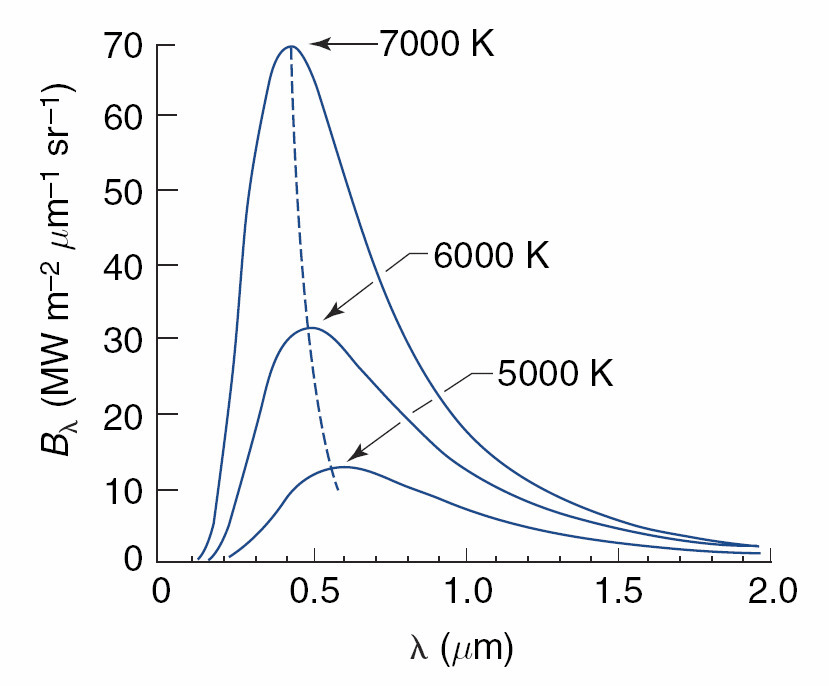
\includegraphics[width=(0.99\linewidth),keepaspectratio]{planckf}
\caption{$B_{\lambda}(T)$ per 3 T.}
\end{figure}

Of two blackbody curves, the one with higher temperature lies entirely above the other:

\begin{align*}
&\PDy{T}{B_{\nu}(T)}=\frac{2h^2\nu^4}{c^2kT^2}\frac{\exp{\frac{h\nu}{kT}}}{[\exp{\frac{h\nu}{kT}}-1]^2}>0\\
&\planckf{\nu}(T\to0)\to0,\ \planckf{\nu}(T\to\infty)\to\infty
\end{align*}

\begin{figure}[!ht]
\centering
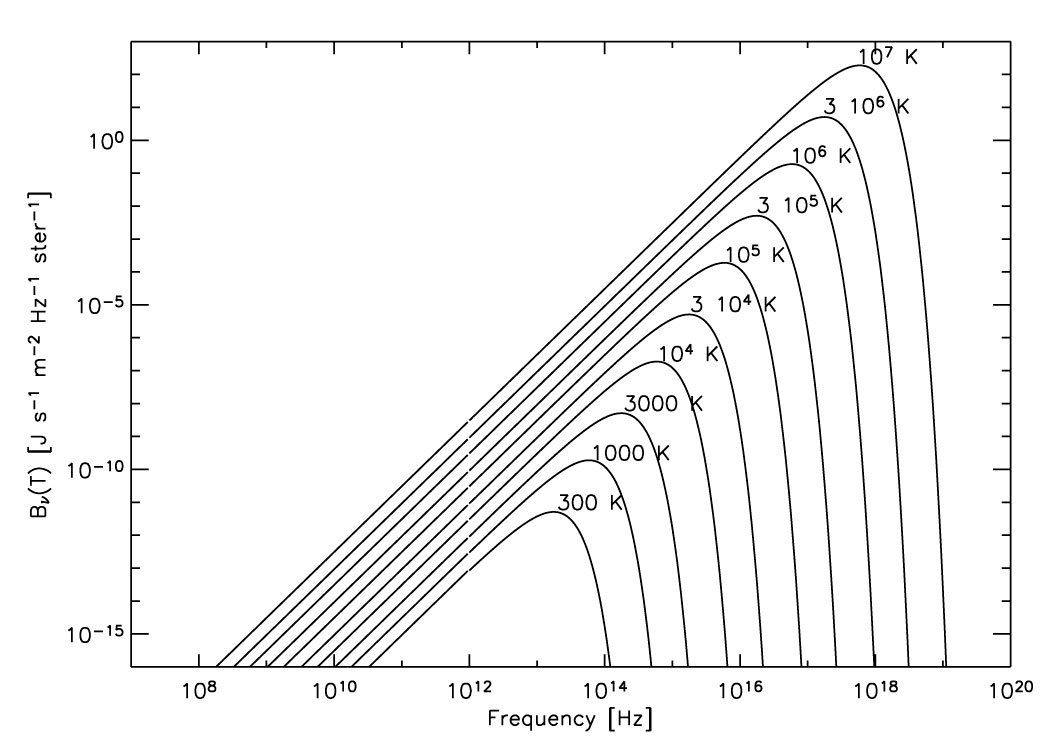
\includegraphics[width=(0.99\linewidth),keepaspectratio]{planckf2}
\caption{Intensit\'a specifica per radiazione di corpo nero in range di T: $\planckf{\nu}(T)$ vs $\nu$.}
\end{figure}

\begin{figure}[!ht]
\centering
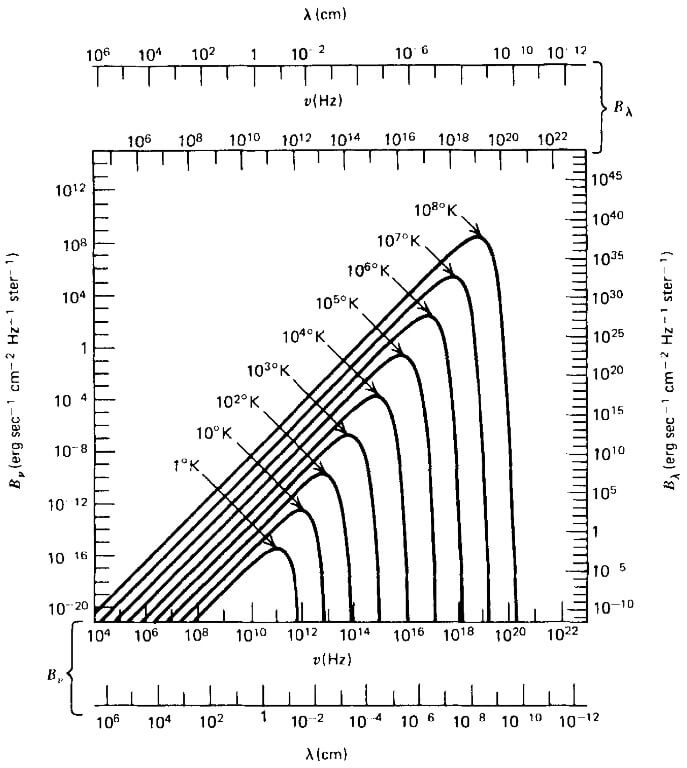
\includegraphics[width=(0.99\linewidth),keepaspectratio]{planckkraus}
\caption{Intensit\'a specifica per radiazione di corpo nero in range di T (cgs). Vedi: Kraus, radio astronomy.}
\end{figure}


\clearpage


\subsection{Energy density of black body radiation.}

\begin{align*}
&u_{\nu}=\frac{4\pi}{c}J_{\nu}\\
&J_{\nu}=\frac{1}{4\pi}\int_{4\pi}\,d\Omega I_{\nu}&\intertext{In thermodynamic equilibrium,}\\
&I_{\nu}=B_{\nu}(T)&\intertext{and is isotropic:}\\
&u_{\nu}=\frac{4\pi}{c}B_{\nu}(T)\\
&u_{\nu}=\frac{8\pi h\nu^3}{c^3}\frac{1}{\exp{\frac{h\nu}{kT}}-1}&\intu{monocromatic energy density of black body radiation.}
\end{align*}

Total energy density:

\begin{align*}
&u=\intzi u_{\nu}\,d\nu=\frac{4\pi}{c}\intzi B_{\nu}(T)\,d\nu\\
&=\frac{4\pi}{c}B(T)\\
&u=\frac{8\pi^5k^4}{15c^3h^3}T^4=aT^4\\
&u=\frac{4\pi}{c}B(T)=\frac{4\pi}{c}\frac{\sigma}{\pi}T^4=aT^4
\end{align*}

\subsection{Radiation pressure.}

In thermodynamic equilibrium (for $\mu_{\nu}=1$), $B_{\nu}=I_{\nu}$ and $I=\intzi I_{\nu}\,d\nu=B(T)$: $B(T)$ is isotropic then $p_r=\frac{1}{3}u$.

\begin{equation*}
p_r=\frac{1}{3}aT^4
\end{equation*}


\section{Degenerate Electron gas.}

\begin{todo}{Degenerate Electron gas}
\end{todo}

\chapter{Legge decadimento radio-attivo}
\PartialToc



\section{Probabilit\'a di decadimento per unit\'a di tempo}
\begin{align*}
&\lambda\\
&=\frac{\text{Probabilit\'a che fra N nuclei 1 decada}}{\text{unit\'a di tempo}}=-\frac{dN}{N}\frac{1}{\text{dt}}
\end{align*}

integro ed ho la legge del decadimento radiativo:
$N(t)=N_0e^{-\lambda t}$.

\section{Attivit\'a}
\begin{align*}
A(t)=\frac{\text{\# decadimenti}}{\text{unit\'a tempo}}=A_0(=\frac{N_0}{\tau})e^{-\lambda t}
\end{align*}

Unit\'a.

Bequerel:
$Bq=\frac{1 \#}{tempo}$.

Curie:
$Ci=3,7 10^{10} \frac{\#}{sec}$.

\section{Vita media}
\begin{align*}
\tau=\frac{\int_0^{\infty}t|\frac{dN}{dt}|dt}{\int_0^{\infty}|\frac{dN}{dt}|dt}
\end{align*}

\section{Tempo di dimezzamento}
$T_{\frac{1}{2}}=\frac{N_0}{2}=N_0e^{-\lambda t_{\frac{1}{2}}}$ cio\'e $t_{\frac{1}{2}}=\tau 0,693$.

\section{Attivit\'a specifica}

Attivit\'a specifica=attivit\'a per unit\'a di massa:

$\lambda\frac{N_A}{A(Numero atomico)}=$.

Attivit\'a emessa durante primo secondo di decadimento di una massa di un grammo.

\section{Branching ratio}

\begin{align*}
&^{40}K\to\\
&\left\{\begin{array}{l} ^{40}Ar \to \lambda_{K,Ar}=0,581 10^{-10} y^{-1} \text{(\Pelectron capture)} \\ ^{40}Ca \to \lambda_{K,Ca}=4,962 10^{-10} y^{-1} \text{(\Pelectron emission)}\\ \end{array} \right.\\
\end{align*}

La probabilit\'a di un decadimento \'e la somma delle ''probabilit\'a parziali'':

\mblock{\lambda_{K,T}=\lambda_{K,Ar}+\lambda_{K,Ca}}

\begin{align*}
&\left\{ \begin{array}{c} ^{40}Ar\\^{40}Ca\\ \end{array} \right\}\\
&= \left\{ \begin{array}{c} ^{40}Ar^0 \\ ^{40}Ca^0 \end{array} \right\}\\
&+ \underbrace{\left\{\begin{array}{c} \frac{\lambda_{K,Ar}}{\lambda_{K,T}}\\ \frac{\lambda_{K,Ca}}{\lambda_{K,T}}\\ \end{array}\right\}}_{\text{Branching ratio}}^{40}K(e^{-\lambda_{k,T}t}-1)
\end{align*}

\section{Total activity of a sample}

The total activity of a sample is the sum of all processes counted per unit of time:

$A=\sum_iA_i=\sum\lambda_in_i$.

\section{Activity of a two elements radioactive chain}

\lbt{N_1(t)=N_0\exp{-\lambda_1 t}}{N_2(t)=N_0\frac{\lambda_1}{\lambda_2-\lambda_1}(\exp{\lambda_1t}-\exp{\lambda_2t})} e \mblock{A_2(t)=\lambda_2N_2(t)=\frac{\lambda_1\lambda_2}{\lambda_2-\lambda_1}(\exp{\lambda_1t}-\exp{\lambda_2t})}

Casi particolari:

\begin{enumerate*}

\item $\lambda_1\ll\lambda_2$ (parent long lived - secular equilibrium).

Approssimo $\exp{-\lambda_1}t\approx1$ quindi \mblock{N_2(t)=N_0\frac{\lambda_1}{\lambda_2}(1-\exp{-\lambda_2 t})}:

as t becomes large nuclei of type 2 are decaying at same rate at which are formed. 


\item $\lambda_1<\lambda_2$ (Transient equilibrium).

Facendo il rapporto fra le attivit\'a
\begin{align*}
\frac{\lambda_2N_2}{\lambda_1N_1}=\frac{\lambda_2}{\lambda_2-\lambda_1}(1-\exp{-(\lambda_2-\lambda_1)t})
\end{align*}

vedo che al crescere di t il rapporto

\begin{align*}
\frac{A_2}{A_1}\abc{\text{t grande}}\frac{\lambda_2}{\lambda_2-\lambda_1}
\end{align*}


\item $\lambda_1>\lambda_2$.

I nuclei parent decadono rapidamente, l'attivit\'a dei nuclei di prima generazione raggiunge un massimo e poi decade con la sua costante caratteristica; $N_2(t)\abc{t\gg\tau_1}N_0\frac{\lambda_1}{\lambda_1-\lambda_2}\exp{-\lambda_2t}$

\end{enumerate*}


\chapter{Onde EM e interazione con materia.}
\PartialToc

\section{Equazioni di Maxwell}

\section{Radiation and equation of radiative equilibrium equilibrium}

\subsection{Radiation.}

\begin{definition}{Specific intensity at P in given direction}
Let $d\sigma$ contain P. At given time there will be rays traversing the surface element in all directions: let us consider specific direction $\hat{s}$. Through every point of $d\sigma$ we can construct cones abutting on $d\sigma$ having axes parallel to $\hat{s}$ direction with solid angles at the apex all equal to definite amount $d\Omega$: this cones define a semi-infinite volume in form of truncated cone.

The radiant energy traversing element of area $d\sigma$ and in volume defined is
\begin{equation*}
I\cos{\theta}\,d\sigma\,d\Omega\,dt
\end{equation*}
where $\theta$ is the angle between the normal to $d\sigma$ and $\hat{s}$ direction.

I is the specific intensity at P in the prescribed direction.
\end{definition}


\begin{definition}{Radiazione omogenea e isotropa.}
$I(P,(\theta,\phi))$ indica l'energia in transito per unit\'a di tempo nel punto P nella direzione definita da $(\theta,\phi)$.

Per radiazione omogenea: \mblock{I(P,(\theta,\phi))=I(P)}.

Per radiazione omogenea e isotropa: \mblock{I(P,(\theta,\phi))=I}.
\end{definition}


\begin{definition}{Flusso radiante attraverso superficie.}
\begin{align*}
&d\Omega=\sin{\theta}\,d\theta\,d\phi&\intd{energy traversing $d\sigma$ in direction defined by $d\Omega$}\\
&I\sin{\theta}\cos{\theta}\,d\theta\,d\phi\,d\sigma\,dt\\
&F=F_+-F_-\\
&=\int_0^{2\pi}\int_0^{\frac{\pi}{2}}I\sin{\theta}\cos{\theta}\,d\theta\,d\phi\\
&+\int_0^{2\pi}\int_{\frac{\pi}{2}}^{\pi}I\sin{\theta}\cos{\theta}\,d\theta\,d\phi
\end{align*}
\end{definition}


\begin{definition}{Densit\'a di energia.}
u \'e la densit\'a di energia radiante cio\'e la quantit\'a di energia per unit\'a di volume in transito per unit\'a di tempo.

u \'e la quantit\'a di energia radiante per unit\'a di volume transiting in the neighborhood of a given point per unit time.

$u_{\nu}\,d\nu$ is the energy density of radiation in interval \mblock{[\nu,\nu+\,d\nu]}.

\begin{align*}
&\frac{1}{c}\iint I\,dV\,d\Omega=\frac{V}{c}\int I\,d\Omega\\
&u=\frac{1}{c}\int\,d\omega I&\intd{per radiazione omogenea:}\\
&u_{\nu}=\frac{4\pi}{c}I_{\nu}\\
&u=\frac{4\pi}{c}I
\end{align*}

\end{definition}

\begin{definition}{emission coefficient}
Consider small element of radiating matter of mass m. The amount of radiating energy emitted in direction specified by $d\Omega$ is
\begin{equation*}
j_{\nu}m\,d\Omega\,dt\,d\nu
\end{equation*}

Necessary condition for $j_{\nu}$ to be isotropic is that mass element is isotropic and is in an isotropic radiation field.

If there are $N_n$ atoms in n state we have
\begin{align*}
&j_{\nu_{nm}}\,d\Omega=\frac{N_n}{\rho}[A_{nm}+B_{nm}I_{\nu_{nm}}h\nu_{nm}\,d\Omega
\end{align*}
\end{definition}


\begin{definition}{Total Absorption coefficient}
A pencil of radiation traversing a medium will be weakened by absorption. Traversing thickness $dr$ the radiation (emergent in phase with incident radiation) changes by
\begin{align*}
&dI_{\nu}=-\kappa_{\nu}\rho I_{\nu}\,dr\\
&I_{\nu}(r)=I_{\nu}(0)\exp{-\int_0^s\kappa_{\nu}\rho\,dr}
\end{align*}
\begin{definition}{Optical depth}
\begin{equation*}
\tau_{\nu}=\int_0^s\kappa_{\nu}\rho\,dr
\end{equation*}
\end{definition}

\end{definition}

\subsection{Radiation pressure}

A quantum of energy $h\nu$ has a momentum $\frac{hy\nu}{c}$ in its direction of propagation. To calculate pressure of radiation at P we have to consider the net rate of transfer of momentum normal to arbitrary surface element $d\sigma$ containing P:
let's consider radiation of frequency $\nu$ incident on surface $d\sigma$ and making angle $\theta$ with the normal, the amount of radiant energy traversing the surface in direction defined by $d\Omega$ is \mblock{I_{\nu}\cos{\theta}\,d\Omega\,d\nu\,d\sigma\,dt} and carries momentum \mblock{\frac{1}{c}I_{\nu}\cos{\theta}\,d\Omega\,d\nu\,d\sigma\,dt} hence normal component of momentum transfer across $d\sigma$ by radiation is
\begin{equation*}
\frac{1}{c}\,d\sigma\,dtI_{\nu}\cos^2{\theta}\,d\Omega\,d\nu
\end{equation*}
hence
\begin{equation*}
p_{rad}(\nu)=\frac{1}{c}\int_0^{2\pi}\int_0^{\pi}I_{\nu}\cos^2{\theta}\sin{\theta}\,d\theta\,d\phi
\end{equation*}

For isotropic radiation field
\begin{align*}
p_{rad}(\nu)=2\pi I_{\nu}\frac{1}{c}\int_0^{\pi}\cos^2{\theta}\sin{\theta}\,d\theta=\frac{4}{3c}\pi I_{\nu}=\frac{1}{3}u_{\nu}
\end{align*}

and, generally,

\begin{equation*}
P_{rad}=\frac{1}{c}\int I\cos^2{\theta}\,d\Omega
\end{equation*}

\subsection{Steady set up in a static medium in LTE.}

For LTE we have $\frac{j_{\nu}}{\kappa_{\nu}}$ depends only on T and $\frac{j_{\nu}}{\kappa_{\nu}}=B_{\nu}(T)$ specific intensity emitted by a black surface.

Equation of transfer
\begin{align*}
&\TDy{s}{I_{\nu_{nm}}}=N_n(A_{nm}+B_{nm}I_{\nu_{nm}})h\nu_{nm}\\
&-N_mB_{mn}h\nu_{nm}I_{\nu_{nm}}\\
&\TDy{s}{I_{\nu_{nm}}}\frac{1}{\rho}=\frac{N_nA_{nm}h\nu_{nm}}{\rho}\\
&-\frac{N_mB_{mn}h\nu_{nm}}{\rho}(1-\frac{N_nB_{nm}}{N_mB_{mn}})I_{\nu_{nm}}
\end{align*}

$j_{\nu}$ include induced emission, is not a scalar in general but include depends on incident intensity $I_{\nu}$.

\begin{align*}
&\TDy{s}{I_{\nu}}\frac{1}{\rho}=\kappa_{\nu}'B_{\nu}-\kappa_{\nu}'I_{\nu}&\intertext{where}\\
&\kappa_{\nu}'=\kappa_{\nu}(1-\exp{-\frac{h\nu}{KT}})\\
&\frac{N_nB_{nm}}{N_mB_{mn}}=\exp{-\frac{h\nu}{KT}}\\
&(\kappa'=\frac{h\nu}{4\pi}(n_1B_{12}-n_2B_{21}))
\end{align*}


\subsection{Radiative equilibrium and equation of transfer for far interior.}

We shall solve
\begin{equation*}
\TDy{s}{I_{\nu}}\frac{1}{\rho}=\kappa_{\nu}'B_{\nu}-\kappa_{\nu}'I_{\nu}
\end{equation*}
under circumstances applicable in star's interior.

Assumption: static, infinite, LTE medium.

A gram of material generate per unit time an amount of mass $\epsilon_{\nu}\,d\nu$ by processes of irreversible character: heat liberated including net gain of heat per unit mass by ''convection'', ''conduction'' and internal energy converted into heat (see subatomic energy source).

Total spontaneous emission per gram per unit time by element mass at temperature T is $4\pi\kappa_{\nu}'B_{\nu}$.

The total absorption less total induced emission is $\opacitynu{}'\int\intensitynu{}\,d\omega$.

Quindi l'eccesso di emissione sull'assorbimento \'e dato da $\opacitynu{}'\int(\blacknu{}-\intensitynu{})\,d\omega$, e in uno stato stazionario deve essere uguale al calore liberato $\epsilon_{\nu}$:

\begin{equation*}
\opacitynu{}'\int(\blacknu{}-\intensitynu{})\,d\omega=\epsilon_{\nu}
\end{equation*}
che \'e l'equazione dell'equilibrio radiativo.

Esprimo la conservazione dell'energia nella forma
\begin{align*}
&\div{\vec{F}_{\nu}}=\epsilon_{\nu}\rho\\
&\div{\text{Stress tensor}}=-\frac{\opacitynu{}'\rho}{c}\vec{F}_{\nu}
\end{align*}

Detto $\tau_{\nu}=\int\opacitynu{}'\rho\,ds$ ho che
\begin{equation*}
\intensitynu{}=\intzi{}\blacknu{}(-\tau_{\nu})\exp{-\tau_{\nu}}\,d\tau_{\nu}
\end{equation*}
L'intensit\'a specifica in un punto e per direzione data \'e la somma dei contributi di emissione di tutti gli elementi di massa sottostanti.

Assumiamo espansione del tipo:
\begin{equation*}
\blacknu{}(-\tau_{\nu})=\blacknu{}(0)-\tau_{\nu}\TDy{\tau_{\nu}}{\blacknu{}}+\frac{1}{2}\tau_{\nu}^2\TtwoDy{\tau_{\nu}}{\blacknu{}}
\end{equation*}
quindi
\begin{align*}
&\intensitynu{}=\blacknu{}(0)-\Dcvar{\tau_{\nu}\TDy{\tau_{\nu}}{\blacknu{}}}{\tau_{\nu}=0}+\Dcvar{\frac{1}{2}\tau_{\nu}^2\TtwoDy{\tau_{\nu}}{\blacknu{}}}{\tau_{\nu}=0}&\intertext{e segue che}\\
&\intensitynu{}=\blacknu{}-\frac{1}{\opacitynu{}'\rho}\nabla_{\hat{s}}\blacknu{}+\frac{1}{\opacitynu{}'\rho}\nabla_{\hat{s}}(\frac{1}{\opacitynu{}'\rho}\nabla_{\hat{s}}\blacknu{})
\end{align*}

The ratio of successive terms are of order of magnitude $\frac{\epsilon}{\overline{\kappa}B}$: in interior of star
\begin{align*}
&\epsilon\approx\SI{100}{\erg\per\gram\per\second}\\
&\kappa\approx\SI{100}{\square\cm\per\gram}\\
&T\approx\SI{e6}{\kelvin}\\
&\frac{100}{100\frac{\sigma}{\pi}\num{e24}}\approx\num{e-19}
\end{align*}

Quandi per i nostri scopi \'e sufficiente scrivere
\begin{equation*}
\intensitynu{}=\blacknu{}-\frac{1}{\opacitynu{}'\rho}\nabla_{\hat{s}}\blacknu{}
\end{equation*}

da cui

\begin{align*}
&u_{\nu}=\frac{1}{c}\int\intensitynu{}\,d\omega=\frac{4\pi}{c}\blacknu{}\\
&u=\frac{4\pi}{c}B=\frac{4\sigma}{c}T^4=aT^4\\
&\vec{F}_{\nu}=-\frac{4\pi}{3\opacitynu{}'\rho}\nabla\blacknu{}&\intertext{(vedi stress tensor $P_{ij}$)}
\end{align*}

In caso di simmetria sferica
\begin{align*}
&F_r(\nu)=-\frac{c}{\opacitynu{}\rho}\TDy{r}{p_r(\nu)}\\
&F_r=-\frac{c}{\kappa\rho}\TDof{r}(\frac{1}{3}aT^4)\\
&\div{\vec{F}}=\frac{1}{r^2}\TDof{r}(r^2F_r)=\epsilon\rho
\end{align*}

\subsection{Radiative transfer in stellar interior (\sch{}).}

\begin{definition}{Opacity.}
Definisco l'opacit\'a come coefficiente d'assorbimanto per grammo: $\kappa\rho\,dl$ \'e la frazione di energia incidente assorbita in $dl$.
\end{definition}

\begin{usefull}{Nearly isotropic radiation.}
All'interno del Sole $\kappa\rho\approx1$ quindi l'approsimazione di radiazione isotropica \'e accettabile.
\end{usefull}

\begin{definition}{Profondit\'a ottica}
\begin{align*}
dI=-In\sigma\,dr=-I\rho\kappa\,dr=-I\,d\tau&\intertext{I=intensit\'a=energia/sec/$cm^2$}
\end{align*}
\end{definition}

Mostro che la deviazione dall'equilibrio termodinamico necessaria per il trasporto di energia in superficie non influisce in maniera rilevante sulla relazione tra densit\'a di energia della radiazione e temperatura della materia tipica dell'equilibrio termico esatto

\begin{equation*}
u=aT^4
\end{equation*}

\begin{figure}[!ht]
\centering
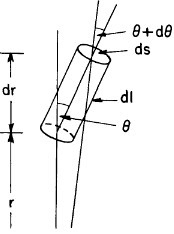
\includegraphics[width=(0.4\textwidth),height=(\textheight-11mm),keepaspectratio]{radiativet}
\caption{Intensity of the radiation field.}
\end{figure}

Geometrical relations
\begin{align*}
&dl=\frac{dr}{\cos{\theta}}\\
&d\theta=-dl\frac{\sin{\theta}}{r}
\end{align*}

Ricavo la relazione esatta tra il flusso di radiazione e il gradiente di temperatura.


Descrivo il campo di radiazione tramite la funzione $I(r,\theta)$ (\si{\erg\per\square\cm\per\second\per\square\radian}) cio\'e l'intensit\'a della radiazione a distanza r dal centro e in direzione inclinata di angolo $\theta$ rispetto a $\vec{r}$.

\begin{align*}
&I(r,\theta)\,d\Omega\,ds-I(r+dr,\theta+d\theta)\,d\Omega\,ds&\intu{gain by radiation entering at bottom surface and loss at top surface}\\
&-I\,d\Omega\,ds*\kappa\rho\,dl&\intu{loss by absorption over the length of the cylinder}\\
&+j\rho\,ds\,dl\frac{d\Omega}{4\pi}&\intu{emission of all matter in the cylinder in direction contained in solid angle $d\Omega$: $j$ rappresenta l'energia emessa da un grammo per secondo in maniera isotropa in tutte le direzioni.}
\end{align*}

\begin{usefull}{Basic equation for radiative transfer.}

\begin{align}\label{eq:radtran}
\PDy{r}{I}\cos{\theta}-\PDy{\theta}{I}\frac{\sin{\theta}}{r}+\kappa\rho I-\frac{1}{4\pi}j\rho=0
\end{align}

\end{usefull}
Fatti:
\begin{itemize}
    \item The equation \ref{eq:radtran} must hold at every points withia a star.
    \item For stellar interior the solution is simplified by the fact that here the radiation field is very nearly isotropic.
\end{itemize}

$I(r,\theta)$ rappresenta la distribuzione di radiazione in tutte le direzioni. Considero i primi momenti di $I$

\begin{align*}
&E(r)=\frac{1}{c}\int I\,d\Omega&\intu{Energy density}\\
&F(r)=\int I\cos{\theta}\,d\Omega&\intu{Radiation flux}\\
&P_R(r)=\frac{1}{c}\int I\cos^2{\theta}\,d\Omega&\intu{Radiation pressure}
\end{align*}

e si ha

\begin{align*}
&\TDy{r}{F}+\frac{2}{r}F+c\kappa\rho u-j\rho=0\\
&\TDy{r}{P_R}+\frac{1}{r}(3P_R-u)+\frac{\kappa\rho}{c}F=0
\end{align*}

\begin{usefull}{quasi-isotropic radiation field: far stellar interio}
Let's represent radiation field at P by
\begin{align*}
&I=I_0+I_1\cos{\theta}+I_2\cos^2{\theta}+\ldots&\intertext{ignoring second term}\\
&\TDy{r}{I_{n-1}}+\kappa\rho I_n=0\\
&|\frac{I_n}{I_{n-1}}|\approx\frac{1}{\kappa\rho R}\approx\num{e-10}
We may restrict to first two terms of the serie
\end{align*}

\end{usefull}

Rappresento il campo di radiazione in un punto tramite la serie

\begin{equation*}
I=I_0+I_1\cos{\theta}+I_2\cos^2{\theta}+\ldots
\end{equation*}

approssimativamente si ha
\begin{equation*}
|\frac{I_n}{I_{n-1}}|\approx\frac{1}{\kappa\rho R}\approx\num{e-10}
\end{equation*}

Inserisco i primi due termini dell'espansione nelle espressioni per i primi momenti di $I$

\begin{align*}
&u=\frac{4\pi}{c}I_0\\
&F=\frac{4\pi}{3}I_1\\
&P_R=\frac{4\pi}{3c}I_0
\end{align*}

quindi
\begin{equation*}
P_R=\frac{1}{3}u
\end{equation*}

L'espressione per l'emissione \'e composta da un contributo per la normale emissione termica e un contributo uguale alla produzione di energia nucleare per grammo per secondo

\begin{equation*}
j=\kappa acT^4+\epsilon
\end{equation*}

Elimino $\epsilon$ tramite la condizione di equilibrio termico
\begin{equation*}
    \TDy{r}{l(r)}=\epsilon\rho4\pi r^2
\end{equation*}

e ottengo

\begin{equation*}
u=aT^4
\end{equation*}


Questa relazione tra la densit\'a di energia della radiazione e la temperatura della materia \'e la stessa che \'e valida per perfetto equilibrio termico: non \'e modificata dalla piccola anisotropia della radiazione nell'interno stellare.

For radiation pressere we have \mblock{P_{rad}=\frac{a}{3}T^4} quindi
\begin{equation*}
H=-\frac{1}{3\kappa\rho}\TDof{r}(acT^4)
\end{equation*}

\clearpage

\section{Local thermodynamic equilibrium.}


\subsection{Thermodynamic equilibrium}

The matter has the same T: radiation field must be homogeneous and isotropic.

The ratio of the emission to the absorption coeffcient for the radiation of frequency $\nu$ in the interior of a homogeneous isotropic medium adiabatically inclosed is equal to the specific intensity of tghe radiation for frequency $\nu$.

\begin{equation*}
j_{\nu}=\kappa_{\nu}I_{\nu}
\end{equation*}

\subsection{Kirchoff's law}

The intensity of radiation emergent from a black surface is indipendent of direction of radiation

\begin{equation*}
\kappa_{\nu}B_{\nu}=j_{\nu}
\end{equation*}

the intensity $I_{\nu}$ of the radiation emitted by a black surface is indipendent of its nature and is a function only of T.

\begin{usefull}{Legge di Kirchoff}
The ratio $\frac{j_{\nu}}{\kappa_{\nu}}$ of the emission to the absorption coefficient of any body in thermodynamical equilibrium depends on temperature only and is indipendent of nature of the body. $\frac{j_{\nu}}{\kappa_{\nu}}$ is equal to specific intensity of the $\nu$ radiation emitted by black surface $I_{\nu}=B_{\nu}$.
\end{usefull}

\subsection{Radiation in adiabatic inclosure at T.}

\begin{align*}
&u=\frac{4\pi}{c}\intzi{}B_{\nu}\,d\nu=aT^4\\
&B(T)=\intzi{}B_{\nu}(T)\,d\nu=\frac{ac}{4\pi}T^4\\
&B(T)=\frac{\sigma}{\pi}T^4&\intertext{$\sigma=\frac{ac}{4}$ is the radiation constant.}
\end{align*}

From QM
\begin{align*}
&B_{\nu}(T)=\frac{2h\nu^3}{c^2}\frac{1}{\exp{\frac{h\nu}{KT}}-1}\\
&B(T)=\frac{2h}{c^2}\intzi{}\frac{\nu^3}{\exp{\frac{h\nu}{KT}}-1}\,d\nu\\
&=\frac{2h}{c^2}(\frac{KT}{h})^4\intzi{}\frac{x^3}{\exp{x}-1}\,dx&\intertext{posto $x=\frac{h\nu}{KT}$}\\
&\intzi{}\frac{x^3}{\exp{x}-1}\,dx\\
&=\intzi{}x^3\exp{-x}(1+\exp{-x}+\exp{-2x}+\ldots)\,dx\\
&6(1+\frac{1}{2^4}+\frac{1}{3^4}+\ldots)\to\frac{\pi^4}{15}
\end{align*}


\section{Emission/absorption coefficient}


\section{Faraday rotation}

\subsection{Faraday rotation in the interstellar medium}

The effect is imposed on light over the course of its propagation from its origin to the Earth, through the interstellar medium. Here, the effect is caused by free electrons and can be characterized as a difference in the refractive index seen by the two circularly polarized propagation modes. Hence, in contrast to the Faraday effect in solids or liquids, interstellar Faraday rotation ($\beta$) has a simple dependence on the wavelength of light ($\lambda$), namely:

\begin{equation*}
\beta= RM \lambda^2
\end{equation*}

where the overall strength of the effect is characterized by RM, the rotation measure. This in turn depends on the axial component of the interstellar magnetic field $B_{\parallel}$, and the number density of electrons $n_e$, both of which vary along the propagation path. In Gaussian cgs units the rotation measure is given by:

 \begin{align*}
&{\displaystyle \mathrm {RM} ={\frac {e^{3}}{2\pi m^{2}c^{4}}}\int _{0}^{d}n_{e}(s)B_{||}(s)\;\mathrm {d} s} {\mathrm {RM}}\\
&={\frac {e^{3}}{2\pi m^{2}c^{4}}}\int _{0}^{d}n_{e}(s)B_{{||}}(s)\;{\mathrm {d}}s
 \end{align*}

or in SI units:

\begin{align*}
 &RM =\frac{e^{3}}{8\pi^{2}\varepsilon_{0}m^2c^3}\int_0^dn_{e}(s)B_{||}(s)\;ds\\
 &\approx (2.62\times 10^{-13}\,T^{-1})\,\int_0^dn_{e}(s)B_{||}(s)\;ds\\
 &RM=\frac{e^{3}}{8\pi^2\varepsilon_{0}m^2c^3}\int_0^dn_{e}(s)B_{\parallel}(s)\;ds\\
 &\approx (2.62\times 10^{-13}\,T^{-1})\,\int_0^dn_{e}(s)B_{\parallel}(s)\;ds
\end{align*}

where $n_e(s)$ is the density of electrons at each point s along the path, $B_{\parallel}(s)$ is the component of the interstellar magnetic field in the direction of propagation at each point s along the path, $e$ is the charge of an electron; $c$ is the speed of light in a vacuum; $m$ is the mass of an electron; $\epsilon_{0}$ is the vacuum permittivity.

The integral is taken over the entire path from the source to the observer.

Faraday rotation is an important tool in astronomy for the measurement of magnetic fields, which can be estimated from rotation measures given a knowledge of the electron number density. In the case of radio pulsars, the dispersion caused by these electrons results in a time delay between pulses received at different wavelengths, which can be measured in terms of the electron column density, or dispersion measure. A measurement of both the dispersion measure and the rotation measure therefore yields the weighted mean of the magnetic field along the line of sight. The same information can be obtained from objects other than pulsars, if the dispersion measure can be estimated based on reasonable guesses about the propagation path length and typical electron densities. In particular, Faraday rotation measurements of polarized radio signals from extragalactic radio sources occulted by the solar corona can be used to estimate both the electron density distribution and the direction and strength of the magnetic field in the coronal plasma.

\subsection{Faraday rotation in the ionosphere}

Radio waves passing through the Earth's ionosphere are likewise subject to the Faraday effect. The ionosphere consists of a plasma containing free electrons which contribute to Faraday rotation according to the above equation, whereas the positive ions are relatively massive and have little influence. In conjunction with the earth's magnetic field, rotation of the polarization of radio waves thus occurs. Since the density of electrons in the ionosphere varies greatly on a daily basis, as well as over the sunspot cycle, the magnitude of the effect varies. However the effect is always proportional to the square of the wavelength, so even at the UHF television frequency of \SI{500}{\mega\hertz} ($\lambda=\SI{60}{\cm}$), there can be more than a complete rotation of the axis of polarization. A consequence is that although most radio transmitting antennas are either vertically or horizontally polarized, the polarization of a medium or short wave signal after reflection by the ionosphere is rather unpredictable. However the Faraday effect due to free electrons diminishes rapidly at higher frequencies (shorter wavelengths) so that at microwave frequencies, used by satellite communications, the transmitted polarization is maintained between the satellite and the ground.

\subsection{Faraday rotation of semiconductors}

GaAs-Faraday rotation spectrum

Due to spin-orbit coupling, undoped $GaAs$ single crystal exhibits much larger Faraday rotation than glass ($SiO_2$). Considering the atomic arrangement is different along the (100) and (110) plane, one might think the Faraday rotation is polarization dependent. However, experimental work revealed an immeasurable anisotropy in the wavelength range from \SIrange{880}{1600}{\nano\meter}. Based on the large Faraday rotation, one might be able to use $GaAs$ to calibrate the B field of the terahertz electromagnetic wave which requires very fast response time. Around the band gap, the Faraday effect shows resonance behavior.

More generally, (ferromagnetic) semiconductors return both electro-gyration and a Faraday response in the high frequency domain. The combination of the two is described by gyroelectromagnetic media, for which gyroelectricity and gyromagnetism (Faraday effect) may occur at the same time.

\section{Fraunhofer lines}

Linee assorbimento.

\begin{figure}[!ht]
\centering
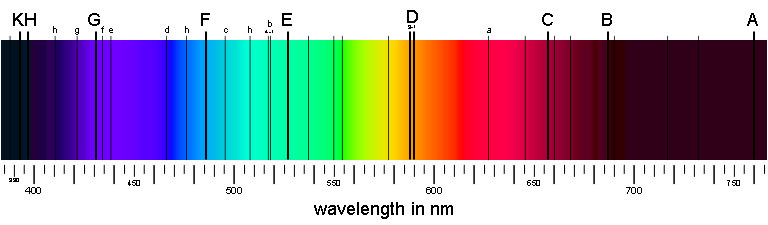
\includegraphics[width=(0.99\textwidth),height=(\textheight),keepaspectratio]{Fraunhofer_lines}
\caption{Linee di Fraunhofer nello spettro solare.}
\end{figure}

\begin{figure}[!ht]
\centering
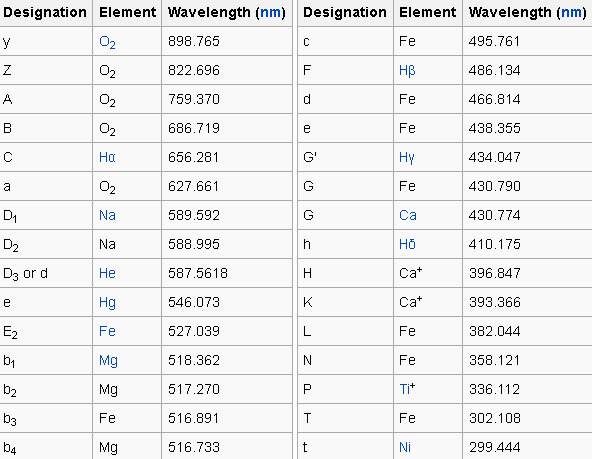
\includegraphics[width=(0.99\textwidth),height=(\textheight),keepaspectratio]{Fraunhoferlambda}
\caption{Lunghezza d'onda delle principali inee di Fraunhofer.}
\end{figure}

\clearpage

\section{Effetto stark}

Classical electrostatics.

The Stark effect originates from the interaction between a charge distribution (atom or molecule) and an external electric field. Before turning to quantum mechanics we describe the interaction classically and consider a continuous charge distribution $\rho(r)$. If this charge distribution is non-polarizable its interaction energy with an external electrostatic potential $V(r)$ is

\begin{align*}
&E_{\mathrm{int}} = \int \rho(\mathbf{r}) V(\mathbf{r}) d\mathbf{r}^3
\end{align*}

If the electric field is of macroscopic origin and the charge distribution is microscopic, it is reasonable to assume that the electric field is uniform over the charge distribution. That is, $V$ is given by a two-term Taylor expansion,

\begin{align*}
&V(\mathbf{r}) = V(\mathbf{0}) - \sum_{i=1}^3 r_i F_i&\intertext{ , with the electric field:}\\
&F_i \equiv -\left. \left(\frac{\partial V}{\partial r_i} \right)\right|_{\mathbf{0}}
\end{align*}

where we took the origin $0$ somewhere within $\rho$. Setting $V(0)$ as the zero energy, the interaction becomes

\begin{align*}
&E_{\mathrm{int}} = - \sum_{i=1}^3 F_i \int \rho(\mathbf{r}) r_i d\mathbf{r} \equiv\\
&- \sum_{i=1}^3 F_i \mu_i = - \mathbf{F}\cdot \boldsymbol{\mu}
\end{align*}

Here we have introduced the dipole moment $\mu$ of $\rho$ as an integral over the charge distribution. In case $\rho$ consists of $N$ point charges $q_j$ this definition becomes a sum

\begin{align*}
&\boldsymbol{\mu} \equiv \sum_{j=1}^N q_j \mathbf{r}_j.
\end{align*}

Perturbation theory.

It is interesting to note that astronomical perturbation applied to a classical hydrogen atom produces a distortion of the electron orbit in a direction perpendicular to the applied electric field.

This effect can be shown without perturbation theory using the relation between the angular momentum and the Laplace-Runge-Lenz vector. Using the Laplace-Runge-Lenz approach, one can see both the transverse distortion and the usual Stark effect. The transverse distortion is not mentioned in most textbooks. This approach can also lead to an exactly solvable approximate model Hamiltonian for an atom in a strong oscillatory field. ''There are few exactly-solvable problems in quantum mechanics, and even fewer with a time-dependent Hamiltonian''

Turning now to quantum mechanics an atom or a molecule can be thought of as a collection of point charges (electrons and nuclei), so that the second definition of the dipole applies. The interaction of atom or molecule with a uniform external field is described by the operator

\begin{align*}
&    V_{\mathrm{int}} = - \mathbf{F}\cdot \boldsymbol{\mu}
\end{align*}.

This operator is used as a perturbation in first- and second-order perturbation theory to account for the first- and second-order Stark effect.
First order

Let the unperturbed atom or molecule be in a g-fold degenerate state with orthonormal zeroth-order state functions \mblock{\psi^0_1, \ldots, \psi^0_g} . (Non-degeneracy is the special case g = 1). According to perturbation theory the first-order energies are the eigenvalues of the g x g matrix with general element

\begin{align*}
&(\mathbf{V}_{\mathrm{int}})_{kl} = \langle \psi^0_k | V_{\mathrm{int}} | \psi^0_l \rangle = -\mathbf{F}\cdot \langle \psi^0_k | \boldsymbol{\mu} | \psi^0_l \rangle, \qquad k,l=1,\ldots, g
\end{align*}
. 

If $g = 1$ (as is often the case for electronic states of molecules) the first-order energy becomes proportional to the expectation (average) value of the dipole operator $\boldsymbol{\mu}$,

\begin{align*}
&E^{(1)} = -\mathbf{F}\cdot \langle \psi^0_1 | \boldsymbol{\mu} | \psi^0_1 \rangle = -\mathbf{F}\cdot \langle \boldsymbol{\mu} \rangle.
\end{align*}

Because a dipole moment is a polar vector, the diagonal elements of the perturbation matrix Vint vanish for systems with an inversion center (such as atoms). Molecules with an inversion center in a non-degenerate electronic state do not have a (permanent) dipole and hence do not show a linear Stark effect.

In order to obtain a non-zero matrix Vint for systems with an inversion center it is necessary that some of the unperturbed functions $\psi^0_i$ have opposite parity (obtain plus and minus under inversion), because only functions of opposite parity give non-vanishing matrix elements. Degenerate zeroth-order states of opposite parity occur for excited hydrogen-like (one-electron) atoms. Such atoms have the principal quantum number n among their quantum numbers. The excited state of hydrogen-like atoms with principal quantum number n is n2-fold degenerate and

\begin{align*}
&n^2 = \sum_{\ell=0}^{n-1} (2 \ell + 1)
\end{align*}, 

where $\ell$ is the azimuthal (angular momentum) quantum number. For instance, the excited n = 4 state contains the following $\ell$ states,

\begin{align*}
&16 = 1 + 3 + 5 +7\ \\
&\Rightarrow\  n=4\hbox{contains}\; s\oplus p\oplus d\oplus f
\end{align*}. 

The one-electron states with even $\ell$ are even under parity, while those with odd $\ell$ are odd under parity. Hence hydrogen-like atoms with n>1 show first-order Stark effect.

The first-order Stark effect occurs in rotational transitions of symmetric top molecules (but not for linear and asymmetric molecules). In first approximation a molecule may be seen as a rigid rotor. A symmetric top rigid rotor has the unperturbed eigenstates

\begin{align*}
&|JKM \rangle = (D^J_{MK})^*\\
&M,K= -J,-J+1,\dots,J 
\end{align*}

with $2(2J+1)$-fold degenerate energy for $|K| > 0$ and $(2J+1)$-fold degenerate energy for $K=0$. Here DJMK is an element of the Wigner D-matrix. The first-order perturbation matrix on basis of the unperturbed rigid rotor function is non-zero and can be diagonalized. This gives shifts and splittings in the rotational spectrum. Quantitative analysis of these Stark shift yields the permanent electric dipole moment of the symmetric top molecule.

\section{Thomson scattering (Coherent Compton effect)}

Thomson scattering cross section valid for \mblock{\frac{h\nu}{m_ec^2}\ll1,\ \lambda\gg\SI{0.02}{\angstrom}}: radiation emitted by oscillating electron with same frequency of impinging EM wave. The energy radiated in unit time by electron whose acceleration is of magnitude a (speed less than c) is \mblock{\TDy{t}{E}=\frac{2}{3}\frac{e^2}{c^3}a^2} with
\begin{equation*}
a=-\frac{eE}{m_e}=-(\frac{eE_0}{m_e})\sin{\omega t}
\end{equation*}

The rate of flow of incoming EM energy across unit area is given by Poynting vector (gaussian unit)
\begin{align*}
&\vec{j}=\frac{c}{4\pi}\vecp{E}{H}\\
&j=\frac{c}{4\pi}E_0^2\sin^2{\omega t}
\end{align*}

The Thomson scattering cross section is
\begin{align*}
&\sigma_0=\frac{\TDy{t}{E}}{j}=\frac{8\pi}{3}a_0^2\\
&=\SI{0.6652e-24}{\square\cm}&\intertext{$a_0=\frac{e^2}{m_ec^2}$ \'e il raggio classico dell'elettrone.}
\end{align*}

\section{Livelli atomici}

\subsection{Energie di ionizzazione}

\begin{align*}
&\SI{13.5984}{\ev}:\chem{^1H}I\to\chem{^1H}II\\
&\SI{24.5873}{\ev}:\chem{^4He}I\to\chem{^4He}II\\
&\SI{54.4177}{\ev}:\chem{^4He}II\to\chem{^4He}III\\
&\SI{7.9024}{\ev}:\chem{_{26}Fe}I\to\chem{_{26}Fe}II\\
&\SI{7.6462}{\ev}:\chem{_{12}Mg}I\to\chem{_{12}Mg}II\\
&\SI{6.1131}{\ev}:\chem{_{20}Ca}I\to\chem{_{20}Ca}II
\end{align*}

\section{Zeeman splitting}

The Zeeman effect can be interpreted in terms of the precession of the orbital angular momentum vector in the magnetic field, similar to the precession of the axis of a spinning top in a gravitational field. 

\subsection{Theoretical presentation}

The total Hamiltonian of an atom in a magnetic field is

\begin{equation*}
H = H_0 + V_M
\end{equation*} 

where $H_0$ is the unperturbed Hamiltonian of the atom, and $V_M$ is the perturbation due to the magnetic field:

\begin{equation*}
V_M = -\vec{\mu} \cdot \vec{B},
\end{equation*}

where $\vec{\mu}$ is the magnetic moment of the atom. The magnetic moment consists of the electronic and nuclear parts; however, the latter is many orders of magnitude smaller and will be neglected here. Therefore,

\begin{equation*}
\vec{\mu} \approx -\frac{\mu_B g \vec{J}}{\hbar},
\end{equation*}

where $\mu_B$ is the Bohr magneton, $\vec{J}$ is the total electronic angular momentum, and g is the Land\'e g-factor. A more accurate approach is to take into account that the operator of the magnetic moment of an electron is a sum of the contributions of the orbital angular momentum $\vec{L}$ and the spin angular momentum $\vec{S}$, with each multiplied by the appropriate gyromagnetic ratio:

\begin{equation*}
\vec{\mu} = -\frac{\mu_B (g_l \vec{L} + g_s \vec{S})}{\hbar}
\end{equation*}

where \mblock{g_l = 1 and g_s \approx 2.0023192} (the latter is called the anomalous gyromagnetic ratio; the deviation of the value from 2 is due to the effects of quantum electrodynamics). In the case of the LS coupling, one can sum over all electrons in the atom:

\begin{equation*}
g \vec{J} = \left\langle\sum_i (g_l \vec{l_i} + g_s \vec{s_i})\right\rangle = \left\langle (g_l\vec{L} + g_s \vec{S})\right\rangle
\end{equation*}

where $\vec{L}$ and $\vec{S}$ are the total orbital momentum and spin of the atom, and averaging is done over a state with a given value of the total angular momentum.

\subsection{Proper zeeman effect}

If the interaction term $V_M$ is small (less than the fine structure), it can be treated as a perturbation; this is the Zeeman effect proper. In the Paschen-Back effect, described below, $V_M$ exceeds the LS coupling significantly (but is still small compared to $H_{0}$). In ultrastrong magnetic fields, the magnetic-field interaction may exceed $H_0$, in which case the atom can no longer exist in its normal meaning, and one talks about Landau levels instead. There are, of course, intermediate cases which are more complex than these limit cases.
Weak field (Zeeman effect)

If the spin-orbit interaction dominates over the effect of the external magnetic field, $\vec{L}$ and $\vec{S}$ are not separately conserved, only the total angular momentum \mblock{\vec{J}= \vec{L} + \vec{S}} is. The spin and orbital angular momentum vectors can be thought of as precessing about the (fixed) total angular momentum vector $\vec{J}$. The (time-)"averaged" spin vector is then the projection of the spin onto the direction of $\vec{J}$:

\begin{equation*}
\vec{S_{avg}} = \frac{(\vec{S} \cdot \vec{J})}{J^2} \vec{J}
\end{equation*}

and for the (time-)"averaged" orbital vector:

\begin{equation*}
    \vec{L_{avg}} = \frac{(\vec{L} \cdot \vec J)}{J^2} \vec{J}
\end{equation*}

Thus,

\begin{equation*}
\langle V_M \rangle = \frac{\mu_B}{\hbar} \vec{J}\left(g_L\frac{\vec{L} \cdot \vec{J}}{J^2} + g_S\frac{\vec{S} \cdot \vec{J}}{J^2}\right) \cdot \vec{B}
\end{equation*}

Using \mblock{\vec{L}= \vec{J} - \vec{S}} and squaring both sides, we get

\begin{equation*}
\vec{S} \cdot \vec{J} = \frac{1}{2}(J^2 + S^2 - L^2) = \frac{\hbar^2}{2}[j(j+1) - l(l+1) + s(s+1)]
\end{equation*}

and: using \mblock{\vec{S}= \vec{J}- \vec{L}} and squaring both sides, we get

\begin{equation*}
 \vec{L} \cdot \vec{J} = \frac{1}{2}(J^2 - S^2 + L^2) = \frac{\hbar^2}{2}[j(j+1) + l(l+1) - s(s+1)]
\end{equation*}

Combining everything and taking \mblock{J_z = \hbar m_j}, we obtain the magnetic potential energy of the atom in the applied external magnetic field,

\begin{align*}
&V_M &= \mu_B B m_j \left[ g_L\frac{j(j+1) + l(l+1) - s(s+1)}{2j(j+1)} + g_S\frac{j(j+1) - l(l+1) + s(s+1)}{2j(j+1)} \right]\\
&= \mu_B B m_j \left[1 + (g_S-1)\frac{j(j+1) - l(l+1) + s(s+1)}{2j(j+1)} \right], \\
&= \mu_B B m_j g_j
\end{align*}

where the quantity in square brackets is the Land\'e g-factor $gJ$ of the atom \mblock{(g_L = 1 and g_S \approx 2)} and $m_j$ is the z-component of the total angular momentum. For a single electron above filled shells $s = 1/2$ and $j = l \pm s$ , the Land\'e g-factor can be simplified into:

\begin{equation*}
g_j = 1 \pm \frac{g_S-1}{2l+1} 
\end{equation*}

Taking $V_m$ to be the perturbation, the Zeeman correction to the energy is

\begin{align*}
&E_Z^{(1)} = \langle nljm_j |H_Z^{'}|nljm_j \rangle\\
&= \langle V_M \rangle_{\Psi} = \mu_B g_J B_{ext} m_j
\end{align*}

Example: Lyman alpha transition in hydrogen

The Lyman alpha transition in hydrogen in the presence of the spin-orbit interaction involves the transitions

\begin{align*}
&2P_{1/2} \to 1S_{1/2}\\
&2P_{3/2} \to 1S_{1/2}
\end{align*}

In the presence of an external magnetic field, the weak-field Zeeman effect splits the $1S1/2$ and $2P1/2$ levels into 2 states each \mblock{(m_j = 1/2, -1/2)} and the $2P3/2$ level into 4 states \mblock{(m_j = 3/2, 1/2, -1/2, -3/2)}. The Land\'e g-factors for the three levels are:

\begin{align*}
&g_J = 2 for 1S_{1/2} (j=1/2, l=0)\\
&g_J = 2/3 for 2P_{1/2} (j=1/2, l=1)\\
&g_J = 4/3 for 2P_{3/2} (j=3/2, l=1)
\end{align*}

Note in particular that the size of the energy splitting is different for the different orbitals, because the $gJ$ values are different. On the left, fine structure splitting is depicted. This splitting occurs even in the absence of a magnetic field, as it is due to spin-orbit coupling. Depicted on the right is the additional Zeeman splitting, which occurs in the presence of magnetic fields.

\subsection{Strong field (Paschen-Back effect)}

The Paschen-Back effect is the splitting of atomic energy levels in the presence of a strong magnetic field. This occurs when an external magnetic field is sufficiently large to disrupt the coupling between orbital ($\vec{L}$) and spin ($\vec{S}$) angular momenta. This effect is the strong-field limit of the Zeeman effect. When $s = 0$, the two effects are equivalent. The effect was named after the German physicists Friedrich Paschen and Ernst E. A. Back.

When the magnetic-field perturbation significantly exceeds the spin-orbit interaction, one can safely assume $[H_{0}, S] = 0$. This allows the expectation values of $L_{z}$ and $S_{z}$ to be easily evaluated for a state $|\psi\rangle$ . The energies are simply

\begin{align*}
&E_{z} = \left\langle \psi \left| H_{0} + \frac{B_{z}\mu_B}{\hbar}(L_{z}+g_{s}S_z) \right|\psi\right\rangle\\
&=E_{0} + B_z\mu_B (m_l + g_{s}m_s)
\end{align*} 

The above may be read as implying that the LS-coupling is completely broken by the external field. However $m_l$ and $m_s$ are still "good" quantum numbers. Together with the selection rules for an electric dipole transition, i.e., \mblock{\Delta s = 0, \Delta m_s = 0, \Delta l = \pm 1, \Delta m_l = 0, \pm 1} this allows to ignore the spin degree of freedom altogether. As a result, only three spectral lines will be visible, corresponding to the \mblock{\Delta m_l = 0, \pm 1} selection rule. The splitting \mblock{\Delta E = B \mu_B \Delta m_l} is independent of the unperturbed energies and electronic configurations of the levels being considered. It should be noted that in general (if $s \neq 0$), these three components are actually groups of several transitions each, due to the residual spin-orbit coupling.

In general, one must now add spin-orbit coupling and relativistic corrections (which are of the same order, known as 'fine structure') as a perturbation to these 'unperturbed' levels. First order perturbation theory with these fine-structure corrections yields the following formula for the Hydrogen atom in the Paschen-Back limit:

\begin{equation*}
E_{z+fs} = E_{z} + \frac{\alpha^2}{2 n^3} \left\{ \frac{3}{4n} - \left[ \frac{l(l+1) - m_l m_s}{l(l+1/2)(l+1) } \right]\right\}. 
\end{equation*}



\section{Scattering/}

Rayleigh scattering applies to the case when the scattering particle is very small (\mblock{x=\frac{2\pi d}{\lambda}\ll1} with a particle size and the whole surface re-radiates with the same phase. Because the particles are randomly positioned, the scattered light arrives at a particular point with a random collection of phases; it is incoherent and the resulting intensity is just the sum of the squares of the amplitudes from each particle and therefore proportional to the inverse fourth power of the wavelength and the sixth power of its size.
 
\subsubsection{From molecules}

The expression above can also be written in terms of individual molecules by expressing the dependence on refractive index in terms of the molecular polarizability $\alpha$, proportional to the dipole moment induced by the electric field of the light. In this case, the Rayleigh scattering intensity for a single particle is given in CGS-units by

\begin{align*}
&I=I_0\frac{8\pi^4\alpha^2}{\lambda^4R^2}(1+\cos^2{\theta})
\end{align*}

\end{document}